\documentclass[bsc, twoside, parskip, abbrevs, notimes, normalheadings,
singlespacing, deptreport]{styles/infthesis}

\usepackage{graphicx}
\graphicspath{ {images/} }

\usepackage{caption}
\usepackage{geometry}

\usepackage[utf8]{inputenc}
\usepackage{array, booktabs}

\usepackage{algorithm2e}
\usepackage{tikz}
\usepackage{listings}

\geometry{left=1.0in,right=1.0in,top=1.0in,bottom=1.0in }


\lstset{
  frame=top,frame=bottom,
  basicstyle=\small\normalfont\sffamily,    % the size of the fonts that are used for the code
  stepnumber=1,                           % the step between two line-numbers. If it is 1 each line will be numbered
  numbersep=10pt,                         % how far the line-numbers are from the code
  tabsize=2,                              % tab size in blank spaces
  extendedchars=true,                     %
  breaklines=true,                        % sets automatic line breaking
  captionpos=t,                           % sets the caption-position to top
  mathescape=true,
  stringstyle=\color{white}\ttfamily, % Farbe der String
  showspaces=false,           % Leerzeichen anzeigen ?
  showtabs=false,             % Tabs anzeigen ?
  xleftmargin=17pt,
  framexleftmargin=17pt,
  framexrightmargin=17pt,
  framexbottommargin=5pt,
  framextopmargin=5pt,
  showstringspaces=false      % Leerzeichen in Strings anzeigen ?
 }
 
\DeclareCaptionFormat{listing}{\rule{\dimexpr\textwidth+17pt\relax}{0.4pt}\par\vskip1pt#1#2#3}
\captionsetup[lstlisting]{format=listing,singlelinecheck=false, margin=0pt, font={sf},labelsep=space,labelfont=bf}

\renewcommand\lstlistingname{Listing}

\DeclareMathVersion{sans}
\SetSymbolFont{operators}{sans}{OT1}{cmbr}{m}{n}
\SetSymbolFont{letters}  {sans}{OML}{cmbrm}{m}{it}
\SetSymbolFont{symbols}  {sans}{OMS}{cmbrs}{m}{n}

\lstnewenvironment{sflisting}[1][]
{\noindent\minipage{\linewidth}\medskip 
   \lstset{basicstyle=\ttfamily\footnotesize,frame=single,#1}}
  {\endminipage}

\lstnewenvironment{mehlisting}[1][]
{\lstset{#1}\mathversion{sans}}{}

\usepackage[round]{natbib}

\usepackage{amsmath}
\usepackage{amsfonts}

\title{StarCraft Brood War as an Agent Learning Platform}
\author{Nantas Nardelli}
\course{Artificial Intelligence and Computer Science}
\project{4th Year Project Report}

\date{\today}

\abstract{

  In the past couple of years the field of Reinforcement Learning has been
  shaken up by what is now labelled as Deep Reinforcement Learning, that is the
  process of using deep architectures such as convolutional neural networks to
  approximate some of the functions required in a reinforcement learning
  process. The shift of part of the community to this particular methodology
  appears to have created the need for test-beds that are unusually more
  data-hungry, data-driven and related to vision or natural language processing.

  Moreover, the inherent hierarchy of those approximation techniques calls for
  advances in Hierarchical Reinforcement Learning. To satisfy these needs we
  have developed a platform for agent learning based on a classic
  Real-Time-Strategy (RTS) game, Starcraft Brood War, and we have built an
  interface to be able to perform experiments based on a popular Deep Learning
  framework, Torch. To test the framework we have then ported the recent
  ``deep'' variant of Q-learning, DQN and made it train on a few simple maps.

  Finally we have started developing an Hierarchical Reinforcement Learning
  algorithm for primitives discovery.

}

\begin{document}

\begin{preliminary}
  \maketitle
  
  \begin{acknowledgements}

To be inserted in paper-ready copy.

\end{acknowledgements}
  
  \standarddeclaration
  
  \dedication{}
  
  \tableofcontents

\end{preliminary}

% outline introduction
% 1. Reinforcement learning introduction
% 2. games as virtual learning environment
% 3. Research approach
% 4. Structure of the Dissertation

\chapter{Introduction}

Artificial Intelligence is an extremely interesting but difficult problem to
address, as research has to at least account for the complexity and breath of
behaviour that has been shown in animals and humans. Autonomy can be sometimes
programmatically engineered, but most of intelligent behaviour requires some
amount of learning that can only be acquired through direct interaction with the
environment, as a big part of being ``intelligent'' has to do with the ability
to generalise knowledge and behave reasonably in unseen scenarios.

\section{Reinforcement Learning}

A technique developed specifically to address this type of learning process is
Reinforcement learning. Reinforcement learning provides a general framework to
learn behaviour in a goal-oriented fashion and without requiring expert
knowledge or labelled data. It is framed to be functional even in situations
where reward is delayed and where environments are not deterministic. Because of
its foundations on dynamic programming, it also allows the use of rich and
powerful mathematical tools for its analysis. Unfortunately those algorithms
learn more or less good behaviour sets only when the environment is sufficiently
tractable, and they start breaking down as the state space increases in size. To
study reinforcement learning we therefore need testbeds that allow to
parametrise the size of this state and that remain interesting enough to provide
challenges for current state-of-the-art algorithms.

\section{Games as Virtual Learning Environments}

The idea of using games as testbeds for Artificial Intelligence is not a new
one. Board games such as Chess, Backgammon and Go have been historically linked
to challenges in AI research, and the AI community has used those games to
compare and study the properties of different algorithms. During the past couple
of decades, the community has gradually ``solved'' or fully tackled those board
games, so part of the community shifted to more complex games, most of which
were popular video games. Those already provided the community a perfect excuse
to study search algorithms and symbolic solvers because of the need to challenge
human players, so it's only natural the gradually got integrated as part of the
testbeds used by researchers working in machine learning and more generally
artificial intelligence.

Reinforcement Learning algorithms have since the beginning found usage when
applied to fields such as robot control, natural language processing and
economics, but most of the theoretical work has required relatively simple and
scalable testbeds to compare algorithms in a systematic and rigorous manner.
Most of those domains were simple adaptations of classical AI problems such as
grid worlds and bandit problems, but as research started getting past those
problems the community had to come up with more structured and complex domains.
Those testbeds have historically mostly consisted of board games like go and
backgammon, but in the past couple of decades the community has also introduced
domains such as simulated football and a variety of video games. All of those share
characteristics that make naive reinforcement learning complex to engineer and
train: they can possess large action or environment state sets, they challenge
algorithms by providing only a degree of partial of observability or they can be
properly solved only by obtaining very strong long-term strategies (that realms
such as planning try to tackle).

% ALE picture here.

A popular and recent learning platform has been for instance the Atari Learning
Environment (ALE), which researchers have mostly used to study reinforcement
learning algorithms that can learn a variety of policies for different games.
Unfortunately the majority of the games contained in this particular
platform don't require anything way more complex than reactive policies, which
means that studying more advanced policy learning on those games has become
quite a forced process.

A category of video games more suitable for providing complex scenarios for
studying RL is the category of Real-Time Strategy (RTS) games. This typology of
games generally requires some amount of long-term planning combined with
interactive and generalisable short-term or reactive planning, and it's
particularly challenging to reinforcement learning algorithms because of the
intrinsic partial observability, the unusually big action space, and its nature
of competitive game. We focus on one of the most popular and still widely played
RTS games, Starcraft.

% cite from http://umichrl.pbworks.com/w/page/7597597/Successes%20of%20Reinforcement%20Learning

\section{Approaching the problem} % TODO rename

The point of this work was primarily about exploring what it would take to
concretely transform and use StarCraft as a platform to study reinforcement
learning and general artificial intelligence. We adopted a scoping approach to
deal with the engineering problem, with the goal to reach a state where we could
successfully run state of the art learning algorithms on StarCraft. This
therefore required the construction of a robust and generic interface to the
game, the creation of an interface to one of the popular tensor libraries and
finally porting and testing a few basic reinforcement learning and deep
reinforcement learning algorithms.

The idea was to prove the feasibility of using StarCraft as a learning platform,
to release the first version of a useful interface to allow the community to
bootstrap work on real time strategy games, and to create a baseline for later
work in the area.

\section{Report Structure}

Chapter 2 presents reinforcement learning and discusses some of the research
done by games. It outlines properties of real time strategy games and it seeks
to explain the benefits of using StarCraft as a research platform. Chapter 3
presents the engineering approach taken and the developed architecture, covering
the entire pipeline from the game to the agent interface, also providing some
example agent learning algorithms. Chapter 4 presents results obtained from
testing the platform using a couple of model-free reinforcement learning
algorithms. Finally Chapter 5 discusses some improvements for the design and
future work.
 % introduction
% outline background

% 1. Video games
% 2. Reinforcement learning
% 3. Deep Reinforcement Learning
% 4. Conclusion

\chapter{Background}

\section{Reinforcement Learning}

\subsection{Markov Decision Processes}

\subsection{Model-free Reinforcement Learning}

\subsection{Hierarchical Reinforcement Learning}

\subsection{Deep Reinforcement Learning}

Deep Reinforcement Learning aims to solve the problem of learning policies from
multi-dimensional state representations without having to manually engineer
features and the representation itself.

\subsubsection{Deep Learning}

\section{Research using games}

\subsection{ALE}

\subsection{RTS AI Research}

\subsection{Using StarCraft as a platform}

\section{Summary}

The first part of this chapter has presented the Reinforcement Learning
framework and the Markov Decision Process, a formalisation that allows to study,
analyse and compare reinforcement learning algorithms. In particular we have
reviewed work in model-free reinforcement learning and research focused on
adding some form of hierarchical structure to reinforcement learning as a way to
address the problem of learning complex policies. Additionally we have looked at
recent work that addresses the problem of learning policies from visual
information using deep learning, a powerful set of algorithms for building
generative models that can automatically discover features and that work
surprisingly well for domains when lots of data is available.

The second part of the chapter has focused on reviewing some of the available
videogame platforms that have successfully been used in artificial intelligence
research, looking in particular at Real-Time Strategy games. Finally we have
provided a description of StarCraft and the rationale behind the idea of
transforming it into a fully-fledged agent learning platform.
 % background
\chapter{Platform Design and Implementation}

As we mentioned in Chapter 1, the goal of this thesis was to develop an
interface for reinforcement learning research in StarCraft. The following
sections outline the process of design, implementation and testing of the
platform.

\section{Specifications}

Obtaining a list of specifications for the platform was relatively challenging
for a few reasons: the design needed to provide a powerful and robust
environment while maintaining a strong degree of expandability. With the sudden
re-popularisation of reinforcement learning the community has begun challenging
previously untouched problems, meaning that entirely new architectures might
soon appear and provide new constraints for existing platforms.

We identified the following minimal requirements:

\begin{itemize}
\item Ability to control StarCraft. This included (but was not limited to)
  starting, pausing, and ending games, killing and re-starting the program,
  selecting certain maps or campaigns.
\item Ability to collect and share game state information.
\item Ability to control the game from the player perspective
\item Ability to collect data from human players and replays available over the
  internet.
\item Ability to use hacks and / or some of the cheats to deactivate some of the
  features that make the general game particularly hard (e.g. fog of war).
\end{itemize}

Additionally the surge of deep reinforcement learning gave us an important
additional requirement: we would need to provide a way to use one or some of the
currently popular deep learning libraries, and a native interface to the visual
output of the game.

\section{Brood War Application Program Interface}

One of the main reasons this project became possible within the given time
constraint was because of the existence of the Brood War Application Program
Interface (BWAPI) \citep{bwapi2011brood}. A closed-source game like StarCraft
would normally be very hard to control and to use as an AI development
framework, but thanks to a few extraordinary developers since 2009 it has been
possible to build bots for the game. BWAPI provides a clean and modular
interface that provides access to the game data structures, allowing to collect
game information and to control units much in the same way a human player would.
Because of its C++ implementation, it's also optimised for speed, however its
design model makes it unfortunately thread-unsafe.

BWAPI uses DLL injection to interact with the game, providing two interfaces to
the game: BWAPIModule and BWAPIClient. The first one allows to control of the
units through callbacks fired by in-game events, so it's mostly suitable for
running agents that do not require to have complete control over the game (as
the game is configured centrally by the injected BWAPI.dll at startup). The
second interface allows to directly connect and interact with the server started
within BWAPI.dll, which gives the ability to arbitrarily control most of the
process state. Even thought BWAPIClient lacked some documentation, we decided to
use it to give us the maximum amount of maneuverability later in the
implementation phase.

\section{Pipeline Design} % 2 pages ()

StarCraft and BWAPI by default are only supported on Windows platforms (We
tested Windows 7, 8 and 10), but most of the critical machine learning and
tensor libraries are actively developed only on Unix systems. While the
situation has gradually seen some improvements with the introduction of CNTK
\citep{dallycntk} and TensorFlow \cite{abaditensorflow} (available on Windows
through Docker), most of the current state-of-the-art development and research
happens on Torch, Theano and Caffe, most of which are widely supported only on
Linux and OS X. Given these constraints we decided to separate our system in two
parts: one running on Windows and directly communicating with StarCraft, and the
other running on Linux and interfacing with one of the mentioned tensor
libraries.

\begin{figure}[h]
    \centering
    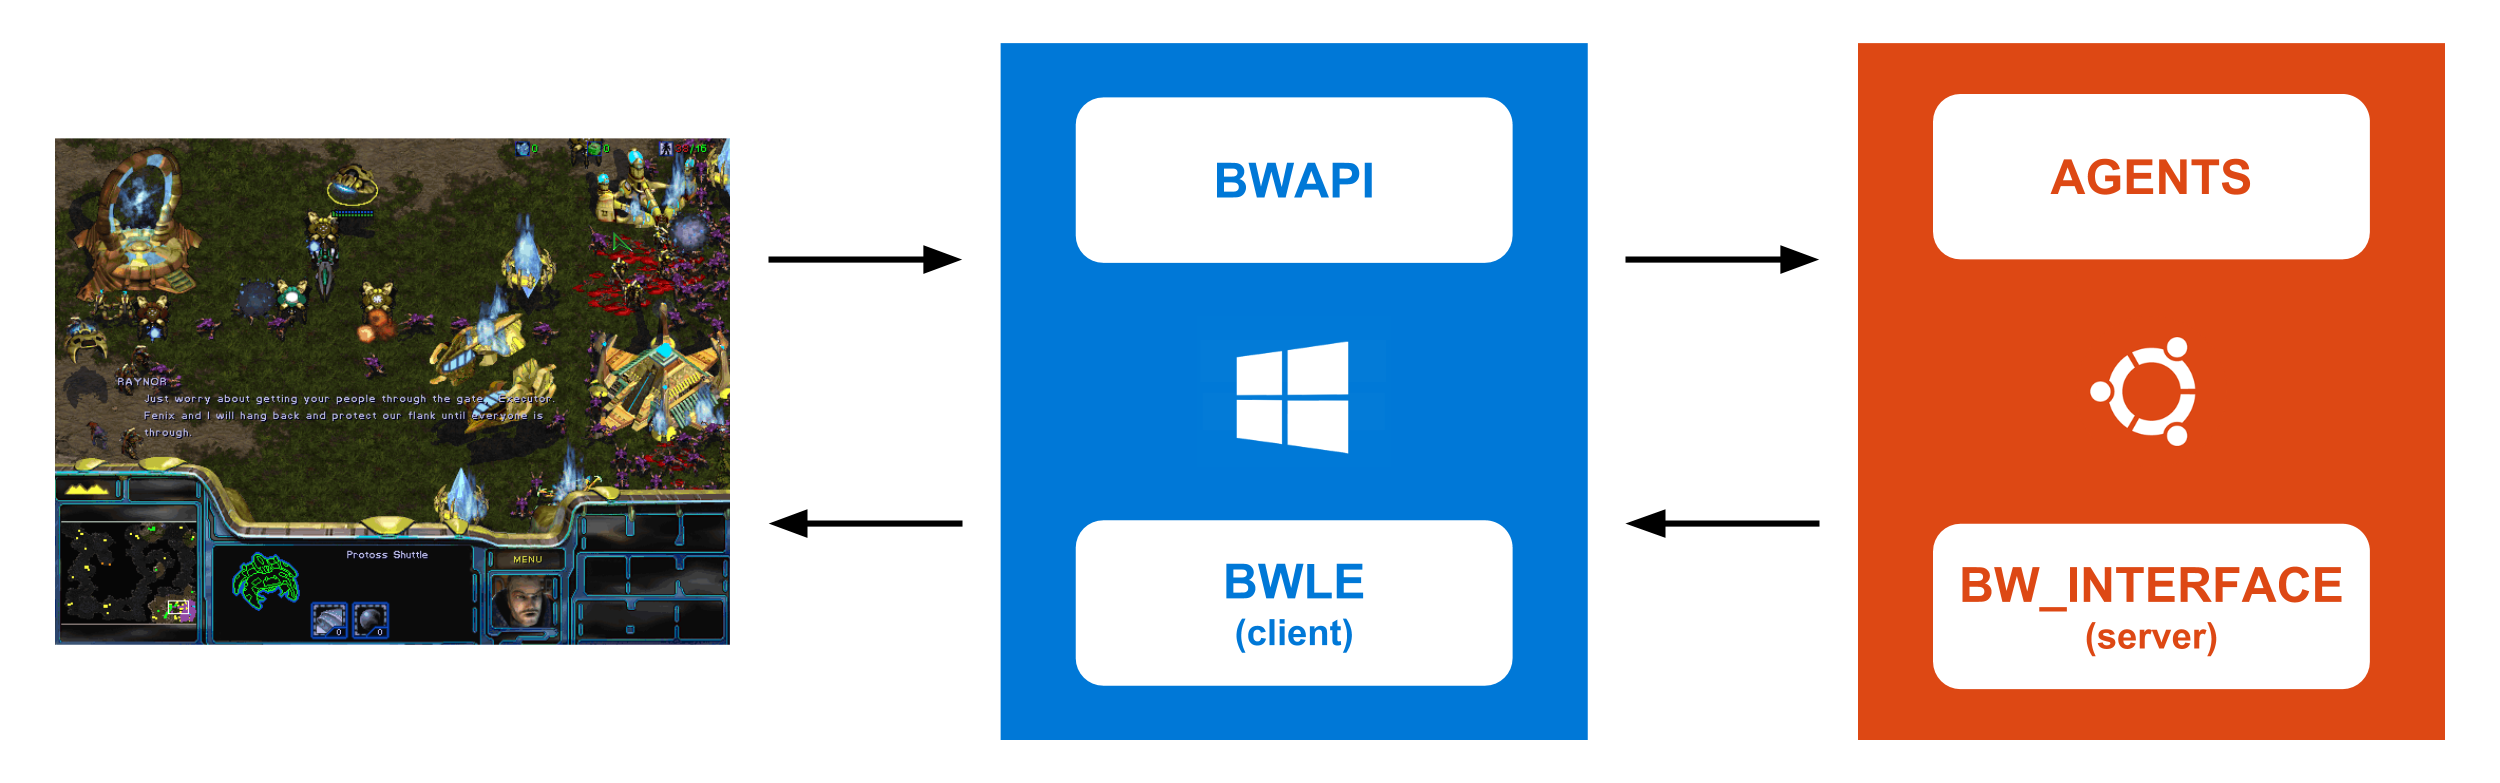
\includegraphics[width=\textwidth]{ch3/arch_overall}
    \caption{Overall architecture. The interface running on Windows 7
      communicates with StarCraft using BWAPI, and connects to a Linux server
      using standard non-blocking sockets. The Linux interfaces communicates
      with an agent through shared objects, }
    \label{fig:arch_ov}
\end{figure}

We designed the systems to communicate between each other using non-blocking TCP
sockets in a synchronous or asynchronous fashion depending on the interface-wide
configuration settings. The choice is dependent mostly on the targeted
experimental setting:

\begin{itemize}
\item synchronous communication can be used to simulate the standard MDP-like
  setting where at each step all agents receive the entirety of all observable
  data, the environment is blocked until the decision process has finished, and
  the environment executes a step when the MDP processes send a certain command.
\item asynchronous communication is instead more useful to have a closer
  simulation to real-world scenarios and games. In this mode the game executes
  each step at a fixed rate and sends information as fast as possible (as the
  game steps rate can be much faster than it's currently possible to process and
  send the visual data). The agent can then send actions at any point of the
  process, which are then executed in the next immediate step.
  This mode is significantly more challenging.
\end{itemize}

To be as efficient and fast as possible, the data structures containing the game
information are serialised using the Google protobuf library
\citep{varda2008protocol}. The library provides a way to generate serialised
objects using pre-defined schemas, which can then be filled with game
information and sent over as compressed strings. Unfortunately the library is
not optimised for very large objects, so in addition to it we implemented our
own serialisation method for sending the image structure over the socket
interface.

While both systems are fully functional, the asynchronous interface requires a
significant amount of work on the agent side to sync the data sources and take
into account the perception/action delay. Such processes are generally
considered a source of research problems but they are not of great interest to
decision making, as once the system is modelled it just becomes part of the
environment.

For the sake of clarity and brevity we will therefore from now on describe the
rest of the system only with respect to the synchronous communication system, as
the implementation of the rest of the modules is mostly independent from this
choice and it greatly simplifies the explanation of the agent interface.

\subsection{Windows Interface}

\begin{figure}[h]
    \centering
    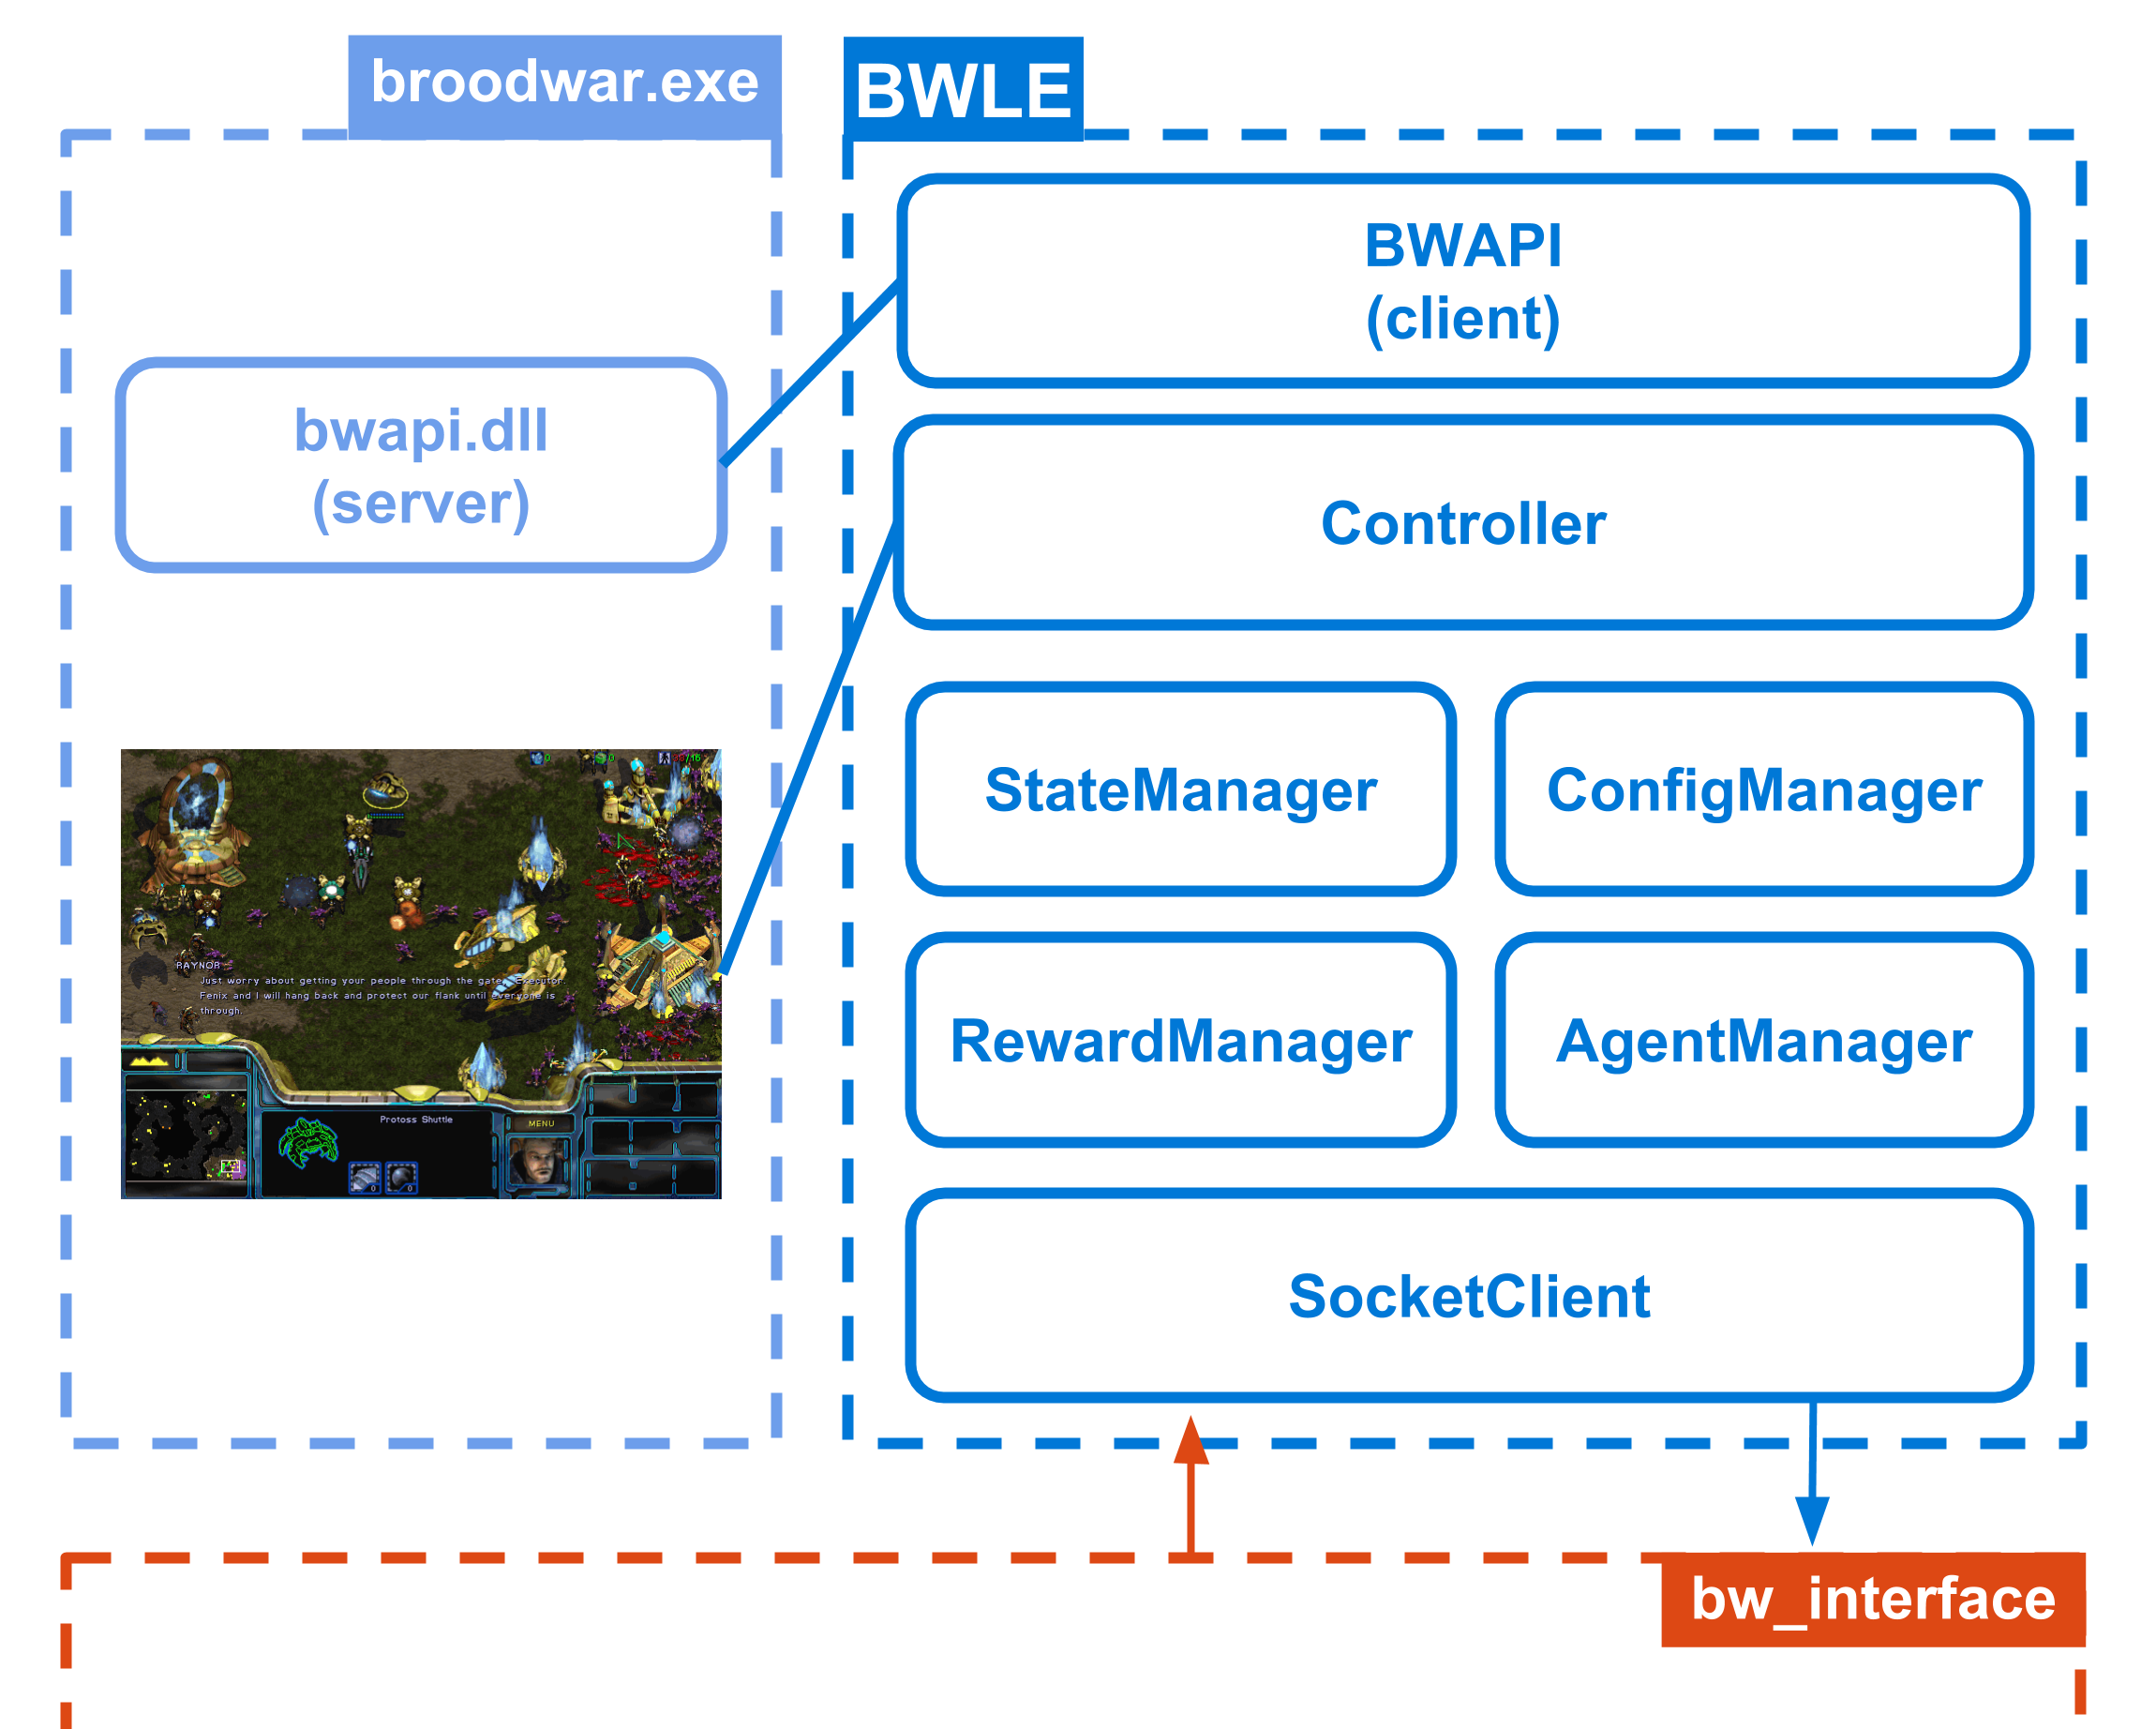
\includegraphics[width=\textwidth]{ch3/arch_win}
    \caption{Overview of the architecture on the Windows sub-system.}
    \label{fig:arch_win}
\end{figure}

To avoid any compatibility problems and to be as fast as possible, we
implemented this side of the architecture in C++ using Windows' Visual C++
compiler. The interface, called \texttt{Brood War Learning Environment} (BWLE)
automatically starts the game, injects \texttt{BWAPI.ddl} and tries to connect
to one of the servers specified in the configuration file(s).

\subsubsection{StarCraft Controller}

Games can be interrupted, terminated or restarted at any time. The client allows
to either completely kill StarCraft, therefore resetting its state with a
process-wide restart, or to just use the in-game restart function to quit the
game and start a new one. The first method allows to change certain settings
that can be loaded only when StarCraft is started, but stops BWAPI for around
two seconds on a quad-core machine between issuing the kill command and the
first step of a new game. The second method allows instead to start a new game
in less than a second. % CITATION NEEDED (check starcraft times)

\begin{sflisting}[caption=Example of a BWLE's configuration file. Fields are not
  mandatory and have reasonable default values. Most of the available options
  are not shown., label=ls:config] 
[standard]
port=12312
address=192.168.0.1
with_image=true
image_skip=0
reward_mode=0
turn_skip=10
map_file=..\share\maps_test_up.txt
map_mode=random
\end{sflisting}

BWLE's configuration system has been written to parse standard INI files,
focusing on completely hiding BWAPI and presenting a unique and coherent
configuration system with useful defaults. A list of maps can then be load in
the system by specifying a file containing a list of files or directories. The
game can also be set to load maps sequentially or in random order, which is an
essential feature for standard training procedures. All the random processes
within BWAPI and the interface can be controlled by specifying a seed at the
start of the experiment. An example configuration can be seen in Listing
\ref{ls:config}.

% TODO: add seed to game if possible, otherwise future work

\subsubsection{Screen capturing}

% TODO describe window size

BWAPI does not provide any interface to capture the visual output of the
game\footnote{Some work had been previously done to integrate some form of
  streaming functionality within BWAPI, but it was dropped in favour of existing
  tools. See https://github.com/bwapi/bwapi/issues/596}, so to fulfill the
specification we developed a module to capture the StarCraft window and include
it in the game state.

To achieve this functionality we use the Graphics Device Interface library
Gdiplus - included as part of the standard Windows Software Development Kit - to
find the StarCraft process, grab an handler to its window, and extract the raw
pixel data. The obtained data structure stores the pixel in an array of 32bit
integers, where integer represent the row-wise RGB data and a null byte.

\begin{figure}[h]
    \centering
    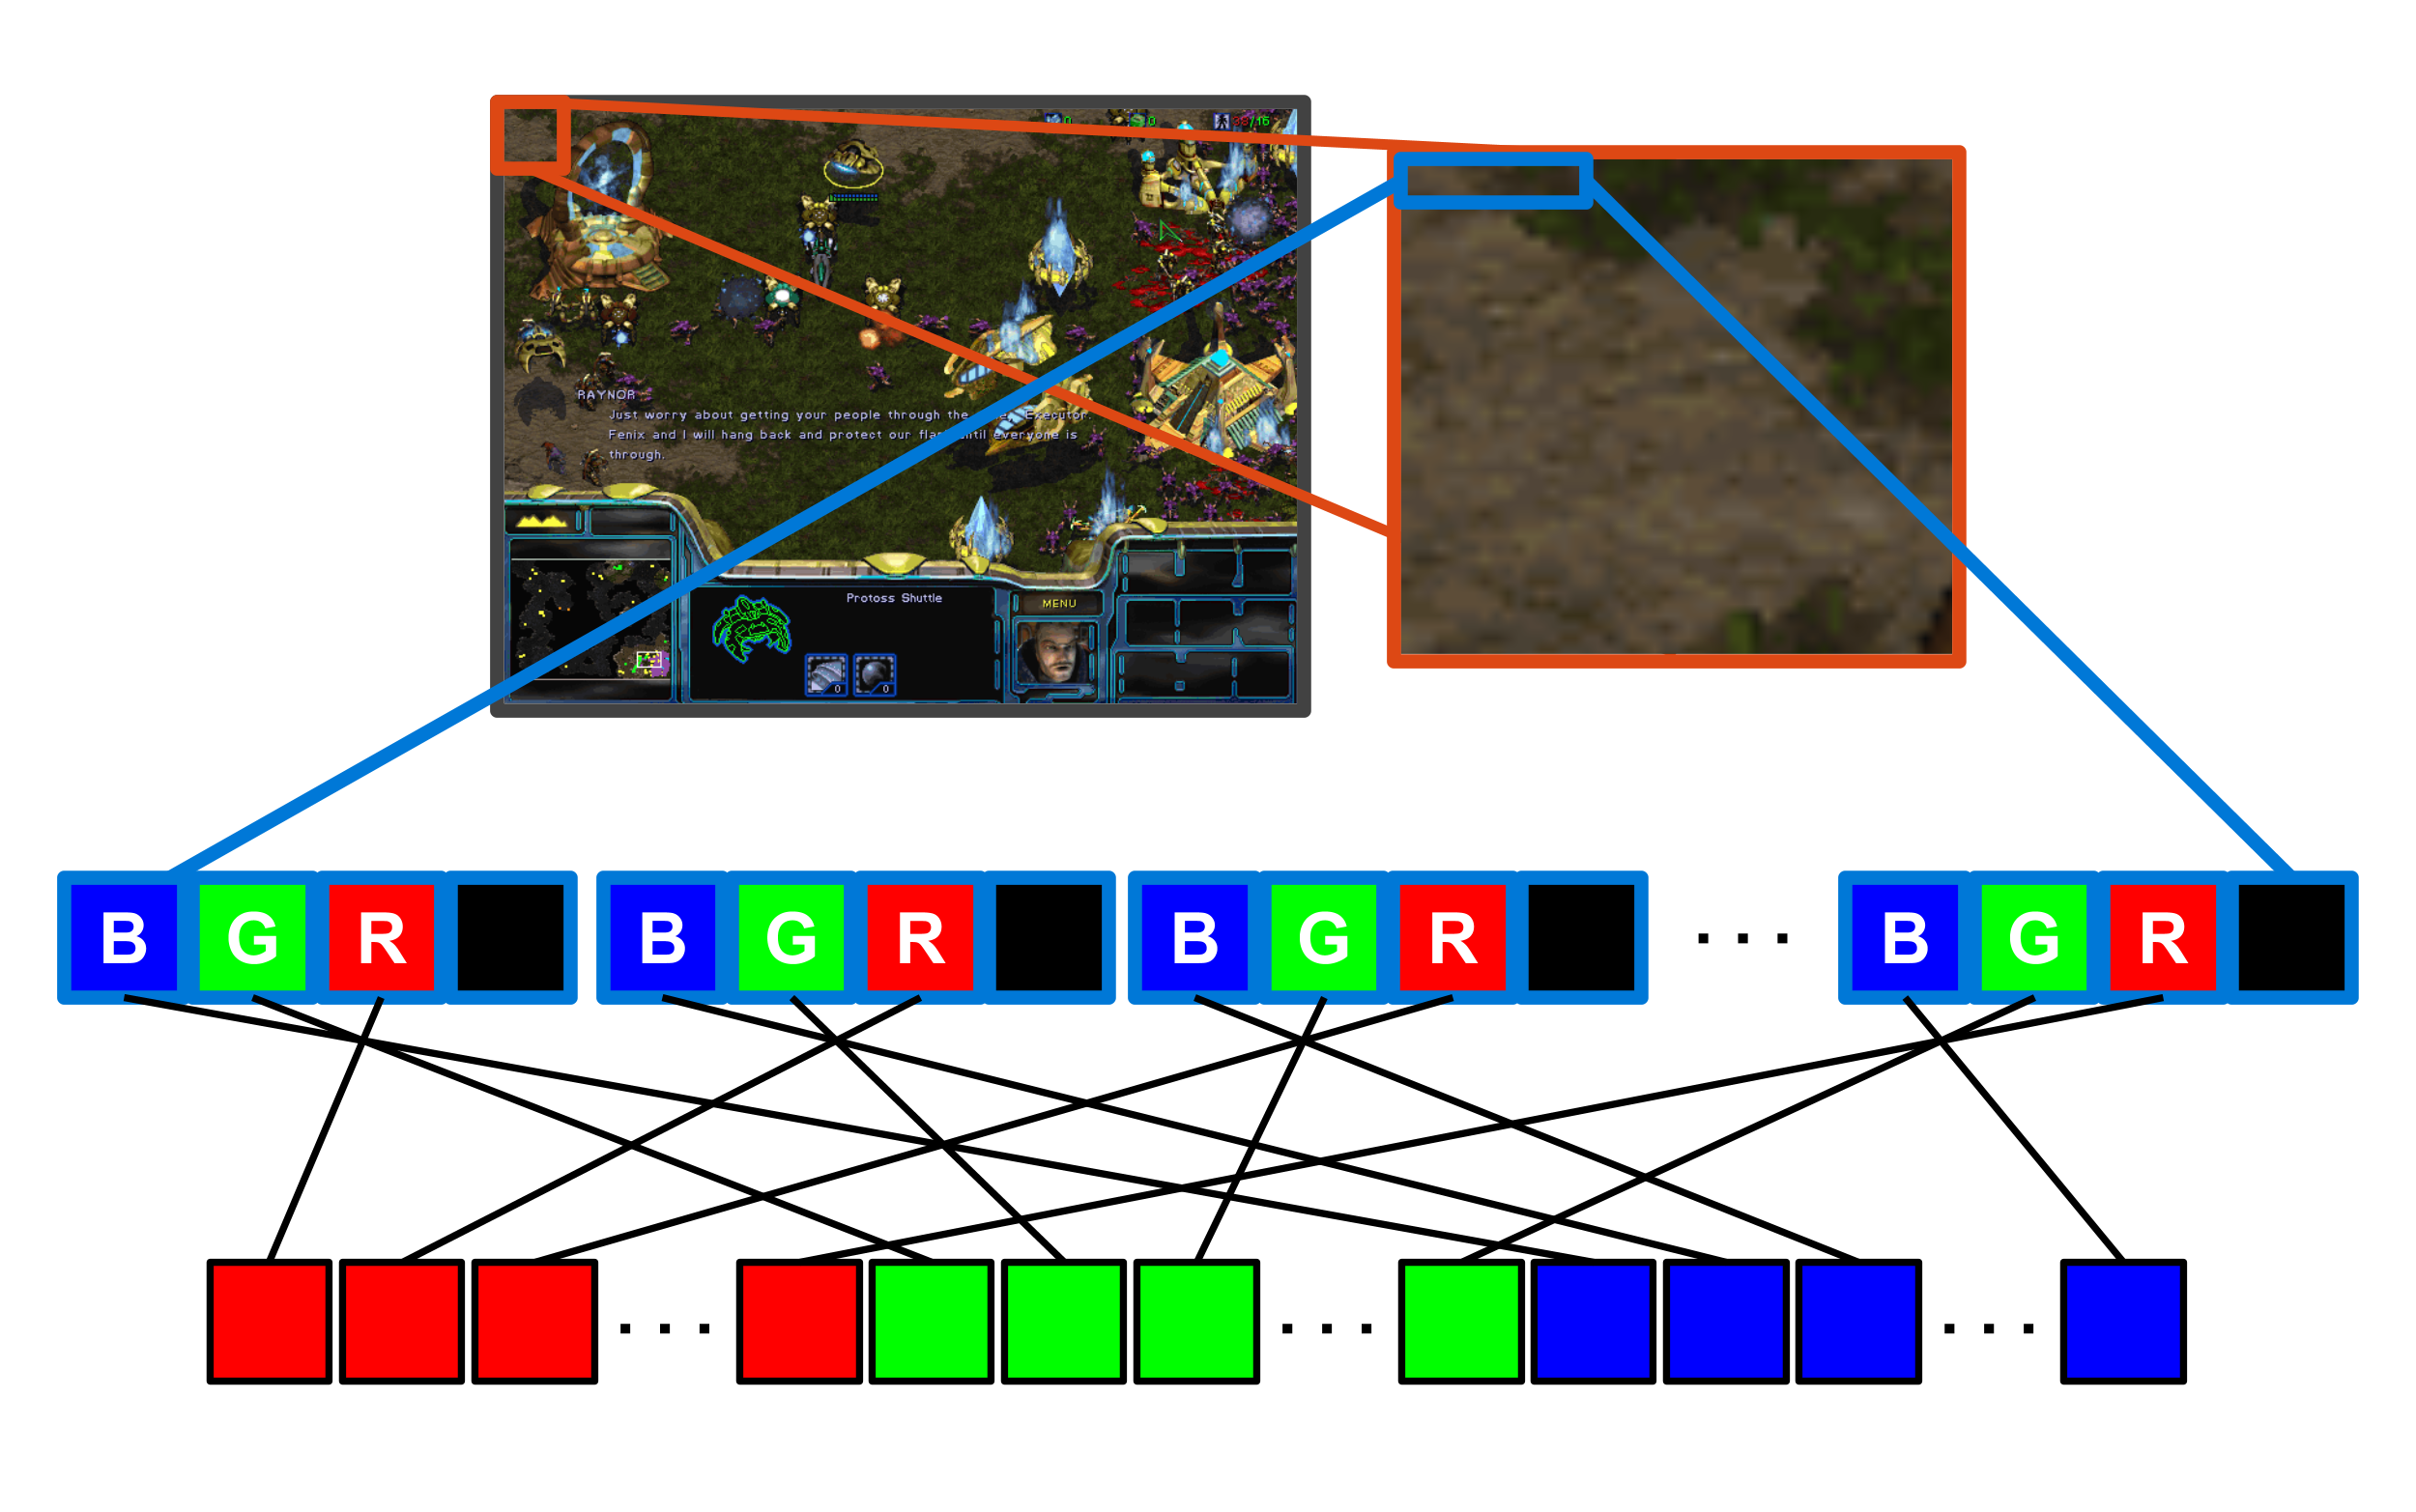
\includegraphics[width=\textwidth]{ch3/capt_conv}
    \caption{Conversion process of the visual data. The raw pixel data captured
      using the window handler gets stripped of superfluous data and separated
      by channel at the same time.}
    \label{fig:capt_conv}
\end{figure}

Before serialising the data to use the network endianness order over the wire,
we strip the null byte and we cluster the channels separately to obtain first
all the red channel values, then the gree channel values, and finally the blue
channel values (Figure \ref{fig:capt_conv}). It must be noted that while this
process has been made as fast as possible on the single thread (given the frame
size), it could be even further optimised by exploiting the fact that the
channels are essentially already independent. 

To allow BWLE to modify the size of the window at running-time we stored all the
captured data using dynamic-size arrays. This required us to add information
such as windows size and bit-dept to the game state data structure so that the
server would be able to calculate the image buffer without making mistakes and
corrupting the data.

% TODO describe image serialisation

\subsubsection{Collecting the Game State}

Collecting the game state also represented a non-trivial design and
implementation challenge. BWAPI was designed with the idea of writing classical
AI bots, not general learning systems. This essentially meant having to deal
with a purposely modular interface split into different objects with respect to
unit classes, weapons, available upgrades, events, forces and so on. The process
of developing a module to collect the game state in a straightforward manner
ended up consisting into many hours of development and testing to learn most of
BWAPI's large functionality. The final outcome was a modifiable query class
\texttt{StateManager} that walks most of the available internal interface while
filtering out errors and unneeded information. Once the module has obtained the
game state, the entirety of the data is loaded into a protobuffer so that it can
be sent over the wire and parsed by the server running on the Linux end.
\texttt{StateManager} is written in such a way that adding units or information
to the unit data structure can be easily achieved by adding entries to the proto
file (which specifies the schema to use to build the C++ interface) and
modifying \texttt{StateManager::setGameState\_} to include the new information
into the protobuffer.

We shaped the design of the module to be purposely centered around the unit data
structure because most of the information available to players is effectively
coupled to the visible units. Everything else can be either inferred or learnt
by playing the game. We have for instance purposely excluded available
information about players, races, and upgrades because they didn't provide any
particularly useful information for our experiments, however it wouldn't take a
huge amount of additional work to identify other useful types of data that
should be included by default in the platform. Part of the \texttt{proto}
specification file can be seen in Listing \ref{ls:proto}

\begin{mehlisting}[caption=Protobuffer schema used to generate the interface used
  to serialise and de-serialise StarCrat's game state., label=ls:proto] 
syntax = "proto2";

enum ActionType {
  ... // The list of action is dependent on the experiment. 
}
enum UnitType {
  ... // Classes of units also dependent on the experiment.
}
message Action {
  required int32 id = 1;
  repeated ActionType action = 2;
}
message Position {
  required int32 x = 1;
  required int32 y = 2;
}
message UnitState {
  required int32 id = 1;
  optional UnitType type = 2;
  optional Position pos = 3;
  optional int32 hp = 4;
  optional bool is_allied = 5;
}
message GameState {
  required bool is_terminal = 1;
  optional int32 last_reward = 2;
  repeated UnitState units = 3;
}
message ImageState {
  required int32 width = 1;
  required int32 height = 2;
  required int32 depth = 3;
}
message ClientPacket {
  required int64 timestamp = 1;
  required bool has_image = 2;
  optional ImageState image_state = 3;
  optional GameState game_state = 4;
}
message ServerPacket {
  optional int64 timestamp = 1;
  optional bool is_training = 2;
  optional bool terminate = 3;
  repeated Action actions = 4; 
}
\end{mehlisting}

\subsubsection{Controlling units}

To centralise the control of units we designed and implemented another manager
module, called \texttt{AgentManager}. Every time a ServerPacket is received the
module extracts the action identifier, the unit associated to the action and any
parameters coupled to it. To allow for non-unit kind of actions, we allowed the
controlled player to correspond to a negative id (-1 by default).
% TODO add parameters to action

One of the main issues of building agents for StarCraft (and most of RTS games)
is that the available actions are entirely context dependent. 
For instance:

\begin{itemize}
\item the generic action \texttt{attack target} becomes \texttt{heal target}
  when the executing unit is a Terran Medic.
\item without workers, a \texttt{mine target} action is completely invalid and
  cannot be executed. That is also the case when workers are present but the
  target is a unit or a building (in which case the action becomes most of the
  times \texttt{attack target}).
\item buildings (and some units) have different upgrades or sometimes no
  available upgrades at all, so a \texttt{upgrade to id} action can have a wide
  variety of effects.
\end{itemize} 

We couldn't find a way to quickly tackle the problem within the project's scope
and time limitation, so we created a few different types of actions based on
some particular scenarios, making sure to designing them to be as general and
reusable as possible. We ended up with three classes of actions:

\begin{description}
\item [Player Actions] - Those actions mostly include game-wide primitives such
  as \texttt{move screen [up|down|left|right]}, and mouse controls such as
  \texttt{click [left|right][pos]} and \texttt{select [area]}.
\item [Basic Unit Actions] - Modelled after GridWorld's actions, those allow the
  agent to move units around the map by specifying either points or vectors.
\item [Complex Unit Actions] - A lot of StarCraft's micro-management can often
  be automatized through interacting with the correct objects in the
  environment. For instance, when a worker is sent to mine it won't be necessary
  to order it to mine close resource areas because the game will automatically
  search for them once the first job is done. Those actions are clearly more
  abstract than basic unit actions, so we felt we needed to include them in a
  separate category. Examples of such implemented actions are in fact
  \texttt{gather closest resource}, and \texttt{attack closest unit}.
\end{description}

To execute some actions the \texttt{Player} module needs the respective action
id and the id of one of the controllable units. Our implementation also allows
to reuse the specified primitive actions by sending multiple action ids within
the packet.
% implemented also into the agents code
% on linux!
Care was taken to make sure that the system was robust enough to ignore killed
or blocked units during the action steps. 

Finally, we can control StarCraft at more than 10Hz, but the game has problems
when the rate of actions-per-minute (APM) is too high, as the game was designed
to handle a maximum of a couple of hundreds APMs. To be able to vary our APM
rate we created a buffer of actions that the agent can use to repeat sent
commands for a fixed number of steps. The number was fixed to simplify the
overall implementation.

% TODO Maybe put a graph?

\subsubsection{Generating Rewards}

Designing the reward scheme of RTS games like StarCraft was another problem that
offered many possible but inter-incomparable (and partial) solutions, making it
problematic to find a generic reward function to cover for all possible in-game
RL sub-problems. When we inspect games played by human players we can
imperically observe that the ideal reward function might in particular need to
be somehow engineered to be hierarchically structured, as the ``goodness'' of a
state-action pair is often entirely context dependent and changes with respect
to a variety of in-game variables. In general this problem is very noticeable
when we look at micro-actions versus strategical moves. Let's look at the
structure of a common competitive game between two players.

It is a widely recognised fact that most board and computer games can be divided
in three major phases, each usually possessing an almost completely isolated
meta-game from the others \citep{liquipediastrat}. Those phases are often called
early-game, mid-game and end-game. In StarCraft, the early game is by design
forcefully dominated by a combination of exploration, resource-gathering and
build-order optimisation. The mid-game is the most variable of the three, and
includes making strategic and tactical decisions to optimise (and protect) a
chosen build-order with respect to a roughly constant resource income rate. This
phase of the game significantly changes depending on the strategy of both
players and the map topology. Finally, the end-game is the last phase of the
game and mostly consists in either the winning player successfully carrying
their final part of the strategy, or the losing player making a comeback thanks
to either errors of the opponent. Similarly to other games and many popular
board games, end-game moves are often carefully-thought and executed, and often
contain some amount of ``gambling'' or decision-making under extreme
uncertainty.

In reality it can also be observed that professional StarCraft players behave
similarly to chess and go players, where the meta-game tends to rely on
particular pre-determined dynamic build-order strategies to choose which tactics
to use when variations of known scenarios appear. At high levels very often the
sequence of actions becomes so close to be optimal (considering human
limitations) that the game effectively is won by which strategy is strong
against the other (in a rock-beat-scissors fashion).

All of those factors contribute in complicating the design of a general purpose
reward system, especially if the final goal is to be able to play good games
against both amateur and professional players. Some research has explored
learning the reward function using techniques like Inverse Reinforcement
Learning\citep{ng2000algorithms}, but none of the explored domains possess state
spaces even remotely comparable StarCraft's.
% TODO Put example image here
To get around the problem we designed a bare-bone module called
\texttt{RewardManager} whose goal mostly consists in analysing the current state
(or a history of the states) and providing a numerical reward. Depending on the
configuration the module can also output a array of values for each unit,
providing support for multi-agent settings or some hierarchical reinforcement
learning methods such as Q-decomposition \citep{russell2003q}. Once the reward
is calculated it's then taken by the \texttt{StateManager} to be inserted into
the protobuffer and sent over to the agent.

% TODO add that more work is needed

\subsection{Linux Interface}

Similarly to the Windows client, the Linux server system was also implemented in
C++. This allowed us to share some of the networking code across the two
modules. We mostly focused on designing a reusable and generic interface, but we
tried to offload most of the decisions involving the domain to the protobuf data
structure and the StarCraft client interface, so that it would later be easier
to link our platform to different language environments or even other games.

One of the main goals we had in mind for this part of the project was in fact to
reach a point in which adapting the interface for any language (or environment)
would become just a matter of defining some symbols and loading a shared object
library. The ability of most mainstream programming languages to load C/C++
symbols either through specific systems such as Foreign Functions Interfaces
(FFIs), or through standard libraries, additionally reinforced our language
decision.

For this project we decided to focus on making an interface exclusively for one
tensor library. We reviewed several environments to take this decision:

\begin{description}
\item [Caffe \citep{jia2014caffe}] - Machine learning library developed by the
  Berkeley Vision and Learning Center. Initially designed purely for computer
  vision research applications, its support for other input types is not
  particularly strong (or is often just absent). It makes heavy use of
  protobuffers to generate neural network architectures and it supports both a
  Python and a C++ interface. One of the most cited reasons for choosing this
  library over the rest is because of the popular Model Zoo: a continuously
  updated collection of trained models from recent NIPS, ICCV and CVPR papers
  that can be all used for comparison purposes.
  
\item [Theano \citep{bergstra2010theano}] - One of the oldest machine learning
  libraries focused on deep learning. Written in Python using numpy to support
  fast mathematical operations, it has spawned several high-level deep learning
  frameworks and is currently one of the most popular tensor libraries. The
  initial design was produce with in mind having to support the variety of use
  cases it later got used for, so the library has grown relatively unevenly,
  making it somewhat bug-prone and difficult to contribute to in comparison to
  other open source libraries.

\item [Torch \citep{collobert2011torch}] - Tensor library written in C and Lua
  mostly used by Facebook, Google DeepMind and a few other companies. It relies
  on LuaJIT, a Just-In-Time interpreter that allows Lua to run at speed
  comparable to pure C code. It has a modular framework that makes it easy to
  develop non-standard layers and architectures. While Lua is a relatively small
  and readable language, its community is small and doesn't compare to the
  Python, C++ or Java communities; this makes the language less attractive as a
  whole for research because of the lack of general-purpose libraries.
\end{description}

We chose Torch because at the time (July 2015) the majority of available Deep
Reinforcement Learning code had been written on top of it. Since then the
available frameworks focused on tensor-based computation and deep learning
nearly doubled (see for instance Microsoft's CNTK, Google's TensorFlow, and
Berkeley's CGT), so the choice would not have been as straightforward had it
been more recent. That said, we still believe our choice to the best one for the
project, considering it effectively forced the C++ interface to be modular right
from the start.
 
\subsubsection{C++ Interface}

\begin{figure}[h]
    \centering
    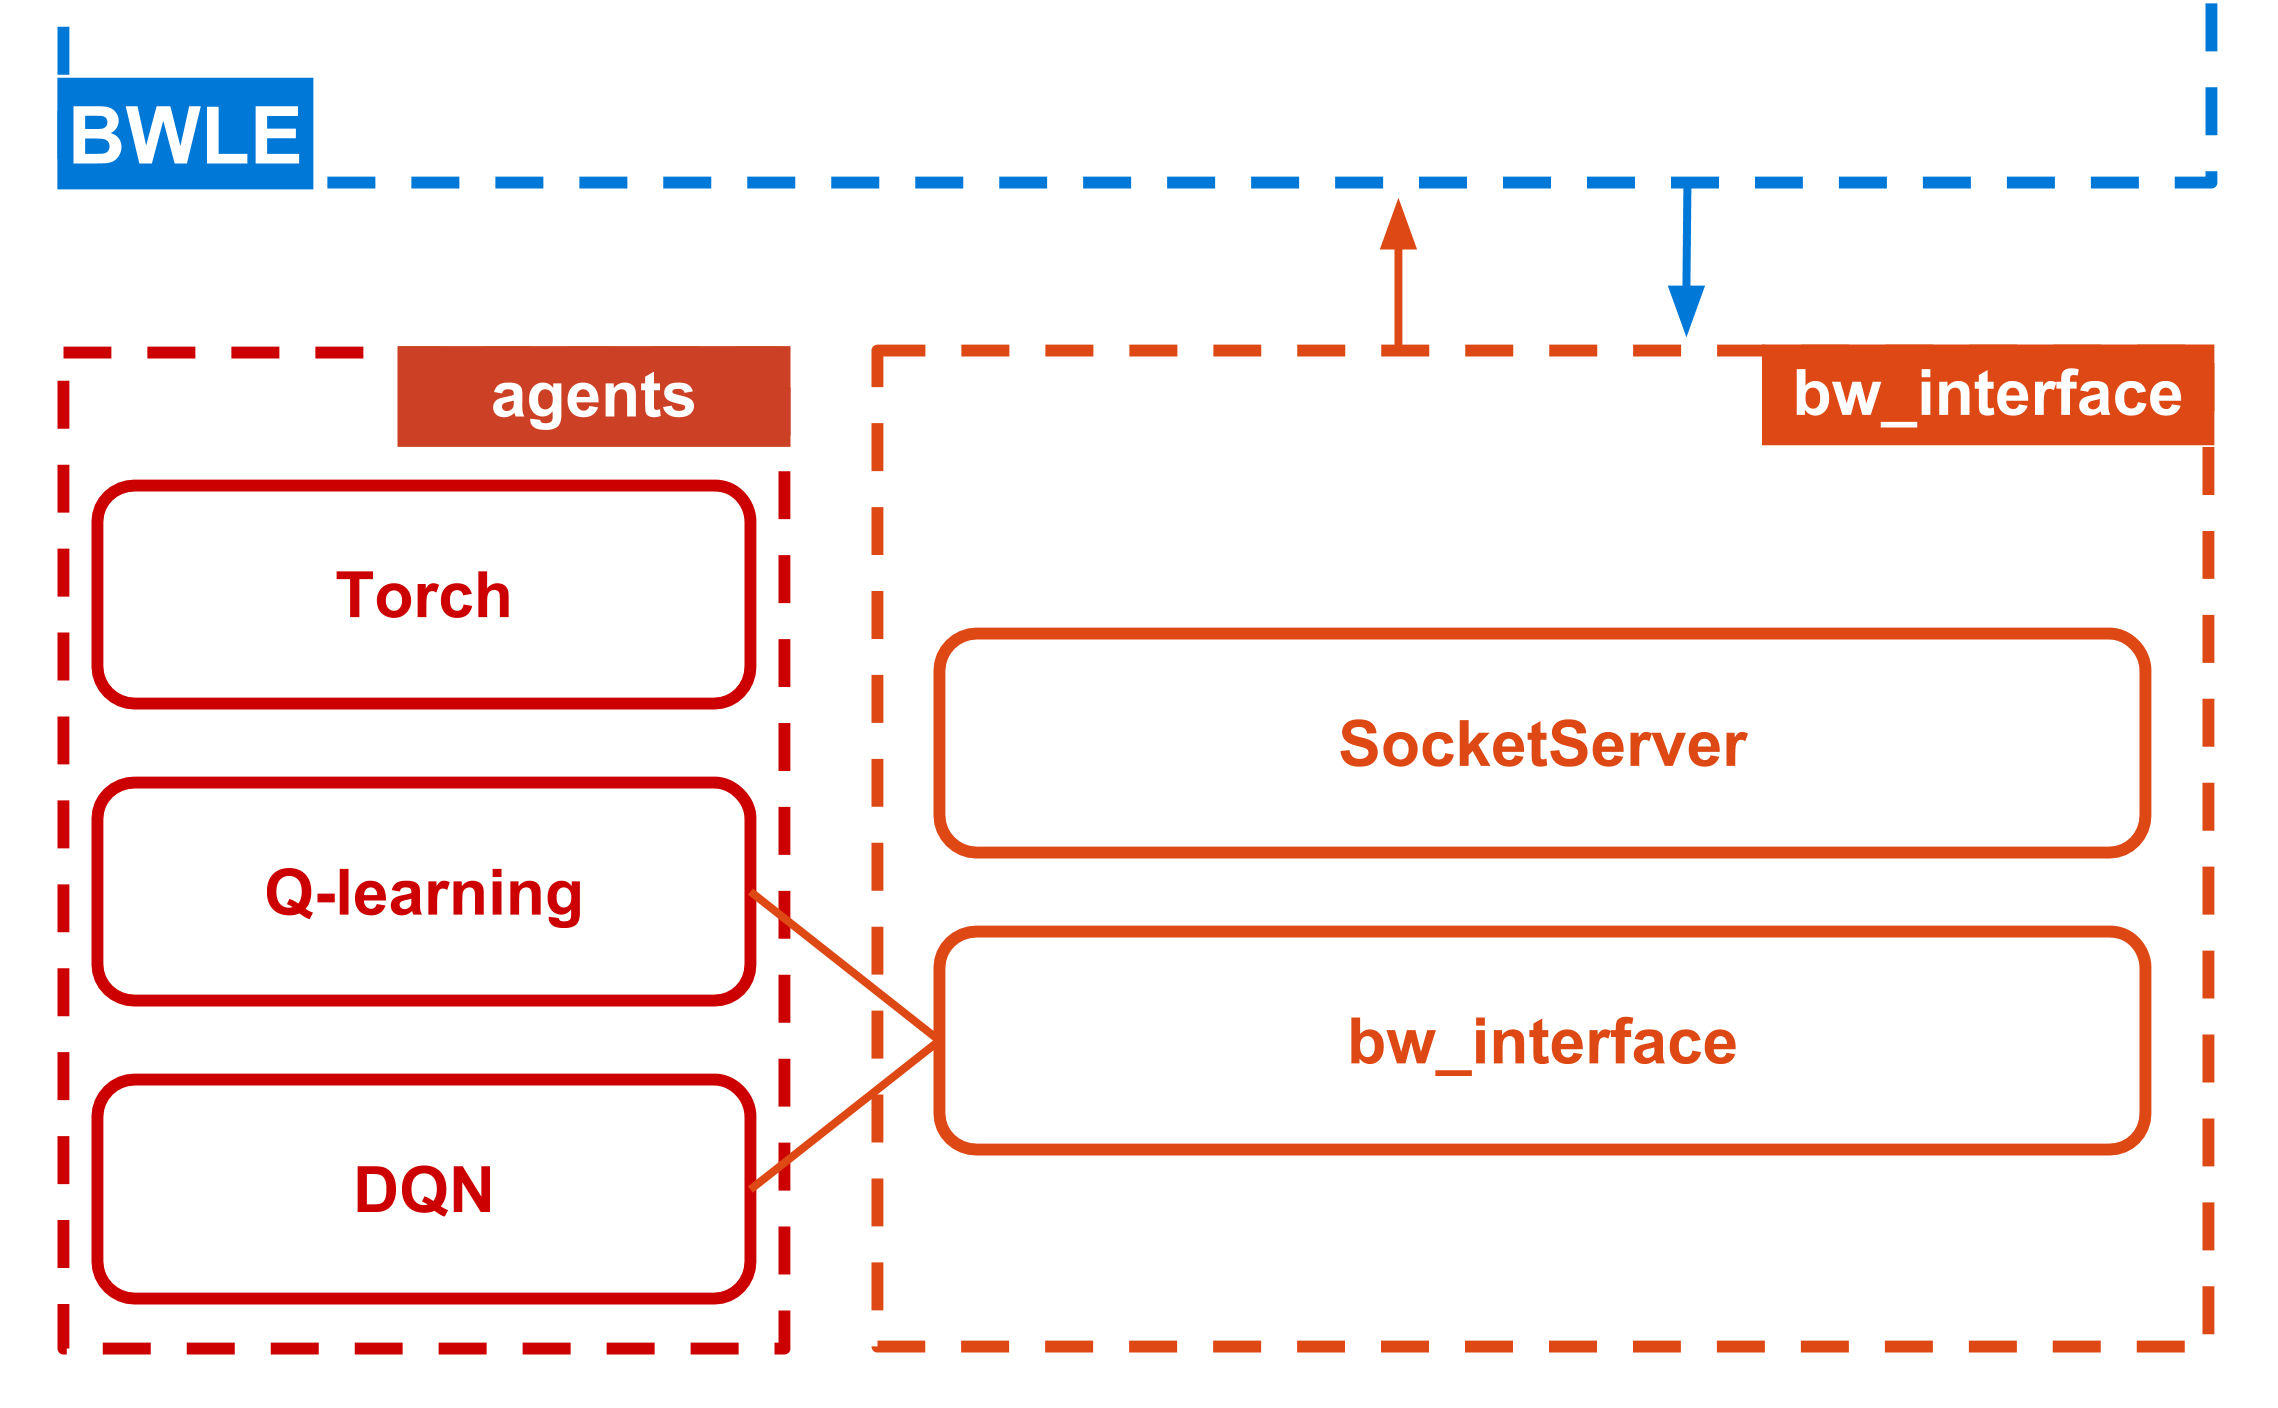
\includegraphics[width=\textwidth]{ch3/arch_linux}
    \caption{Overview of the architecture of the Linux sub-system.}
    \label{fig:arch_linux}
\end{figure}

We designed the Linux C++ interface to be complementary to the Windows client.
The interface started simply as a standard socket server and subsequently
evolved into a fully-fledged controller after adding a protobuffer parser, a
controller class and a storage system. Like the client, the server system
supports both synchronous and asynchronous modes, using non-blocking threaded
TCP sockets.

The overall system is coupled with the client and requires to update the
generated protobuffer interface every time the proto configuration file is
changed on the client side. Because of this we couldn't escape from adding the
library as a dependency, but this update was made painless by scripting the
whole process.

The system is split into three different modules:
\begin{description}
\item [Server] - Manages the connection with the client. It's the first object
  that the interfaces initialises, so it blocks the execution of the process
  until at least a client connects to it. The module was designed from the start
  to support multiple sockets and clients, but we didn't find the time to spin
  more than 2 instances of StarCraft on the cloud and run an heavy stress-test
  for this functionality.
\item [RingBuffer] - To provide a native way of storing and managing long-term
  information received from the client, we implemented a module to act as a
  middle-ware storage system based on a cyclic buffer. The history length can be
  changed when initialised and it's optimised so that the operation of switching
  data around the buffer is as fast as possible (this was done by doing some
  standard pointer manipulation).
\item [BotInterface] - This module essentially acts as the manager class for the
  whole interface. It starts the server, it initialises the data structures for
  the ring buffer and the temporary protobuf parser, and it provides methods to
  interact with the client.
\end{description}

Once we developed and tested the C++ interface, we had to create a LuaJIT
wrapper around it to allow our Lua agents to use it.

\subsubsection{Lua-compatible Interface}

LuaJIT provides an FFI library to wrap C/C++ objects and their interfaces
\citep{pall2008luajit}. The library provides a way to parse C declarations,
which can then be used to read a compiled shared object file containing the C
objects definitions. This allows to integrate C and C++ code (exported as C)
very quickly, without any need to manually write language bindings in Lua. The
Just-In-Time compiler generates instructions that are roughly as efficient
as the ones obtained by standard C compilers like GNU \texttt{gcc} and
\texttt{Clang}.

Arguably the most interesting part about our interface is that it provides a
method to take the raw pixel data sent by client and transform it into a Torch
tensor that can then be used by the Lua agents. This was possible by using the
Torch C API provided with the framework, which allowed us to copy the obtained
from the C heap to the LuaJIT storage system. We therefore became able to treat
our image as a Torch object and take advantage of the provided Torch
\texttt{image} library. We also leveraged the Torch \texttt{cunn} library to
make use of CUDA \citep{nvidia2008programming}, NVIDIA's GPU programming
library. This allowed us to train and test some of our agents on recent GPUs.

\subsubsection{Connecting the agents}

To provide the interface to the agent we used the FFI library to wrap the C++
objects, grouping the resulting functions into a class using Torch's
\texttt{Class} library. The end-result was \texttt{bw\_interface}, a module that agents could include
and use as a standard Lua table. 

We didn't wrap the entirety of the C++ functionality because we decided to
implement the ring buffer functionality in our agents as well, as to match the
common interface available to agents running on ALE for the sake of consistency.
The final accessible version of the interface to the agents ended up containing
a rich interface. Some important functions are for instance:

\begin{description}
\item [send\_packet(void)] - Sends the \texttt{ServerPacket} package to the
  client, allowing to control the execution of the environment.
\item [add\_action(int, int*)] - Takes a unit id and an array of action ids and
  adds it to the list of actions.
\item [get\_image\_tensor(void)] - Returns the last received image as a
  \texttt{DoubleTensor}. The tensor has been constructed in such a way to be
  directly compatible with the standard Torch \texttt{image} library. 
\item [get\_state(void)] - Return the game state as a hierarchical Lua table
  that the agent can walk through by simple recursive exploration of the
  attached dictionary of keys. The \texttt{inspect} library is used to test the
  state to check for possible errors.
\item [step(table, bool)] - In synchronous mode, order the client to update the
  game and perform a step. A step is defined as the amount of turns it takes to
  complete the defined set of actions (which can be a fixed amount).
\item [new\_game(bool)] - Order the game to start a new game and return the
  first state-reward pair.
\end{description}
 
\section{Summary}

In this chapter we have outlined the architecture of our entire system, looking
in particular at the design choices related to each module. We have described
our implementation and delineated some challenging issues when modelling RTS
games in a programmatic fashion.
 % implementation
\chapter{Experimental Methodology} 

Our initial goal was to implement a couple of algorithms as baseline for
experiments outside of the scope of this work. Ideally, those algorithms would
have also helped us finding any ``low-hanging fruits'' to properly start
tackling the entire game as a whole big machine learning problem. In addition to
implementing those algorithms, we also designed a few automatic tests to check
the validity of the game state information in known maps.

\section{Test Task}

We have already mentioned a few times how hard StarCraft becomes when posed as a
machine learning and reinforcement learning problem. \cite{} have shown that a
standard game of StarCraft has a state of approximately $10^{1000}$, which is an
incredibly high number even when compared to the large state spaces of Chess
($10^{50}$ to $10^{120}$ states) and Go ($10^{70}$ to $10^{360}$ states)
\citep{papadimitriou2003computational}. Because of this we never considered
tackling the game a part of this project. However, we decided to create a few
test maps and scenarios to aid debugging and see how reinforcement learning
agents would perform on a reduced StarCraft domain.

\subsection{Navigation Task}

\begin{figure}[h]
    \centering
    
\includegraphics[width=0.9\textwidth]{placeholder}
    \caption{Example of map instance of the navigation task.}
    \label{fig:nav_task}
\end{figure}

We came up with this task by looking at the simplest problem human players have
to solve when playing StarCraft: moving units around the map.

The first sub-problem consisted in checking whether we could learn simple
policies based on location goals. We constructed 20 small maps in which a unit
was spawned on the opposite edge of map from the goal and had to reach the map
in the smallest amount of time. The agent received a reward of -1 for going
further away from the goal and +1 for getting closer to the goal. Reaching the
goal would give 100 of reward and would terminate the trial. You can see some of
those maps in Figure \ref{fig:nav_task}. We disabled \texttt{moveScreen*}
actions for both agents as we made the map small enough for all the relevant
information to be available. The Q-learning agent had access to the goal
position.

\subsection{Guided Navigation Task}

\begin{figure}[h]
    \centering
    
\includegraphics[width=0.9\textwidth]{placeholder}
    \caption{Example of map instance of the guided navigation task.}
    \label{fig:guid_task}
\end{figure}

The second task was a larger variation of the first one in which we also added
``death-zones''. Those zones acted as a repellent for the agents, giving a
reward of -100 when touched and acting as terminal states. The Q-learning agent
was given only one particular map configuration and access to the goal position,
while DQN had 20 maps to learn how to avoid danger maps. To guide the agent
visually we added a thick red border in the direction of the goal and we
assigned a different terrain pattern to the danger-zones. This time the map was
too large to cover the screen, so we locked the window to keep the unit always
at the center of the window. Figure \ref{fig:guid_task} shows an example of one
of those maps.

\subsection{Survival Task}

\begin{figure}[h]
    \centering
    
\includegraphics[width=0.9\textwidth]{placeholder}
    \caption{Example of map instance of the survival task.}
    \label{fig:surv_task}
\end{figure}

Our final task consisted in an interactive navigation problem. In particular,
one or more units was spawned in one of 20 maps in which all the allied units
were either close to aggressive enemy units or partly surrounded by them.
The agent would receive a reward of -10 if any of the units was killed, killing
a unit would account for a reward of 5, and 0 for any other event (or lack
thereof). Because of the multi-dimensionality of the space, it became possible
to receive different rewards at each time, so rewards received at some step $t$
were summed together before being sent to the agent. Figure \ref{fig:surv_task}
shows an example of one of those maps.

\section{RL Algorithms}

At the start of the project we decided that by the end of it we would have two
categories of testing algorithms: a classic model-free RL algorithm to test an
MDP-like setting and the newer DQN, a deep reinforcement learning algorithm, to
test learning policies purely from the visual input.

\subsection{Q-learning}

The choice of Q-learning as the test model-free algorithm was relatively
straightforward: Q-learning \citep{watkins1992q} is one of the most popular and
powerful model-free RL algorithms and it represents the foundation of many other
reinforcement learning algorithms. Given a standard MDP in the form of a tuple
$(S, A, T, R)$ where $S$ is the state space, $A$ is the action space, $T(s, s')$
is the transition probability distribution of moving from state $s$ to state
$s'$, and $R$ is the immediate reward received when moving from state $s$ to
state $s'$, Q-learning allows to iteratively find a policy that maximises the
expected total reward in a trial by learning from experience gained by using
some explorative policy (as opposed to on-policy reinforcement learning where
the policy used to gain ``experience'' is the same as the one that is being
learnt).

In particular, our algorithms works by updating an action-value function $Q(s,
a)$ using an $\epsilon$-greedy policy to gain new samples. Given a learning rate
$\alpha$ and a discount factor $\gamma$,

\begin{equation}
  Q(s_t, a_t) \leftarrow Q(s_t, a_t) +
  \alpha \left[ r_{t+1} + \gamma \max_a Q(s_{t+1}, a) - Q(s_t, a_t) \right].
\label{eq:ql}
\end{equation}

The agent policy in the evaluation phase then becomes

\begin{equation}
  \pi(s, a) = \operatornamewithlimits{argmax}_a Q(s, a).
\label{eq:ql2}
\end{equation}

It has been proved that this policy converges to the optimal policy $\pi*$ given
enough samples from all state-action pairs
\citep{Sutton:1998:IRL:551283}. % TODO how?

The Q function can be represented as a table of values (a simple array) or can
be approximated using a function approximator, however a lot of literature has
highlighted difficulties in making Q-learning (and other model-free RL
algorithms) converge when the action-value function is approximated
\citep{Baird_1997}. In some cases researchers managed to converge the
algorithms, but obtained significantly degraded policies
\citep{bertsekas_1996_tetris, waver_and_baxter_1999, boyan_and_moore_1995}.

\subsubsection{Task dependent state representation}

Providing a state representation for quickly testing the whole system ended up
resulting in a far more challenging problem than initially estimated. To be able
to extensively test the symbolic game state data being sent by the client we
wanted to obtain a useful state representation without having to use a black-box
function approximator such as an artificial neural network, as it would have
made it very hard to do automatic testings. Moreover we wanted to check and
explore how difficult it would have been to use standard RL techniques on
StarCraft's large state space.

\begin{figure}[h]
    \centering
    
\includegraphics[width=0.9\textwidth]{placeholder}
    \caption{Example of a state in our test domain.}
    \label{fig:sample_state}
\end{figure}

Figure \ref{fig:sample_state} shows a sample of the game state data in our
domain. We can see that it is difficult to represent such a representation in an
array because the data increases with the number of units. To create a
representation that we can use in a tabular fashion we must at least manually
compress the state in some way.

\begin{figure}[h]
    \centering
    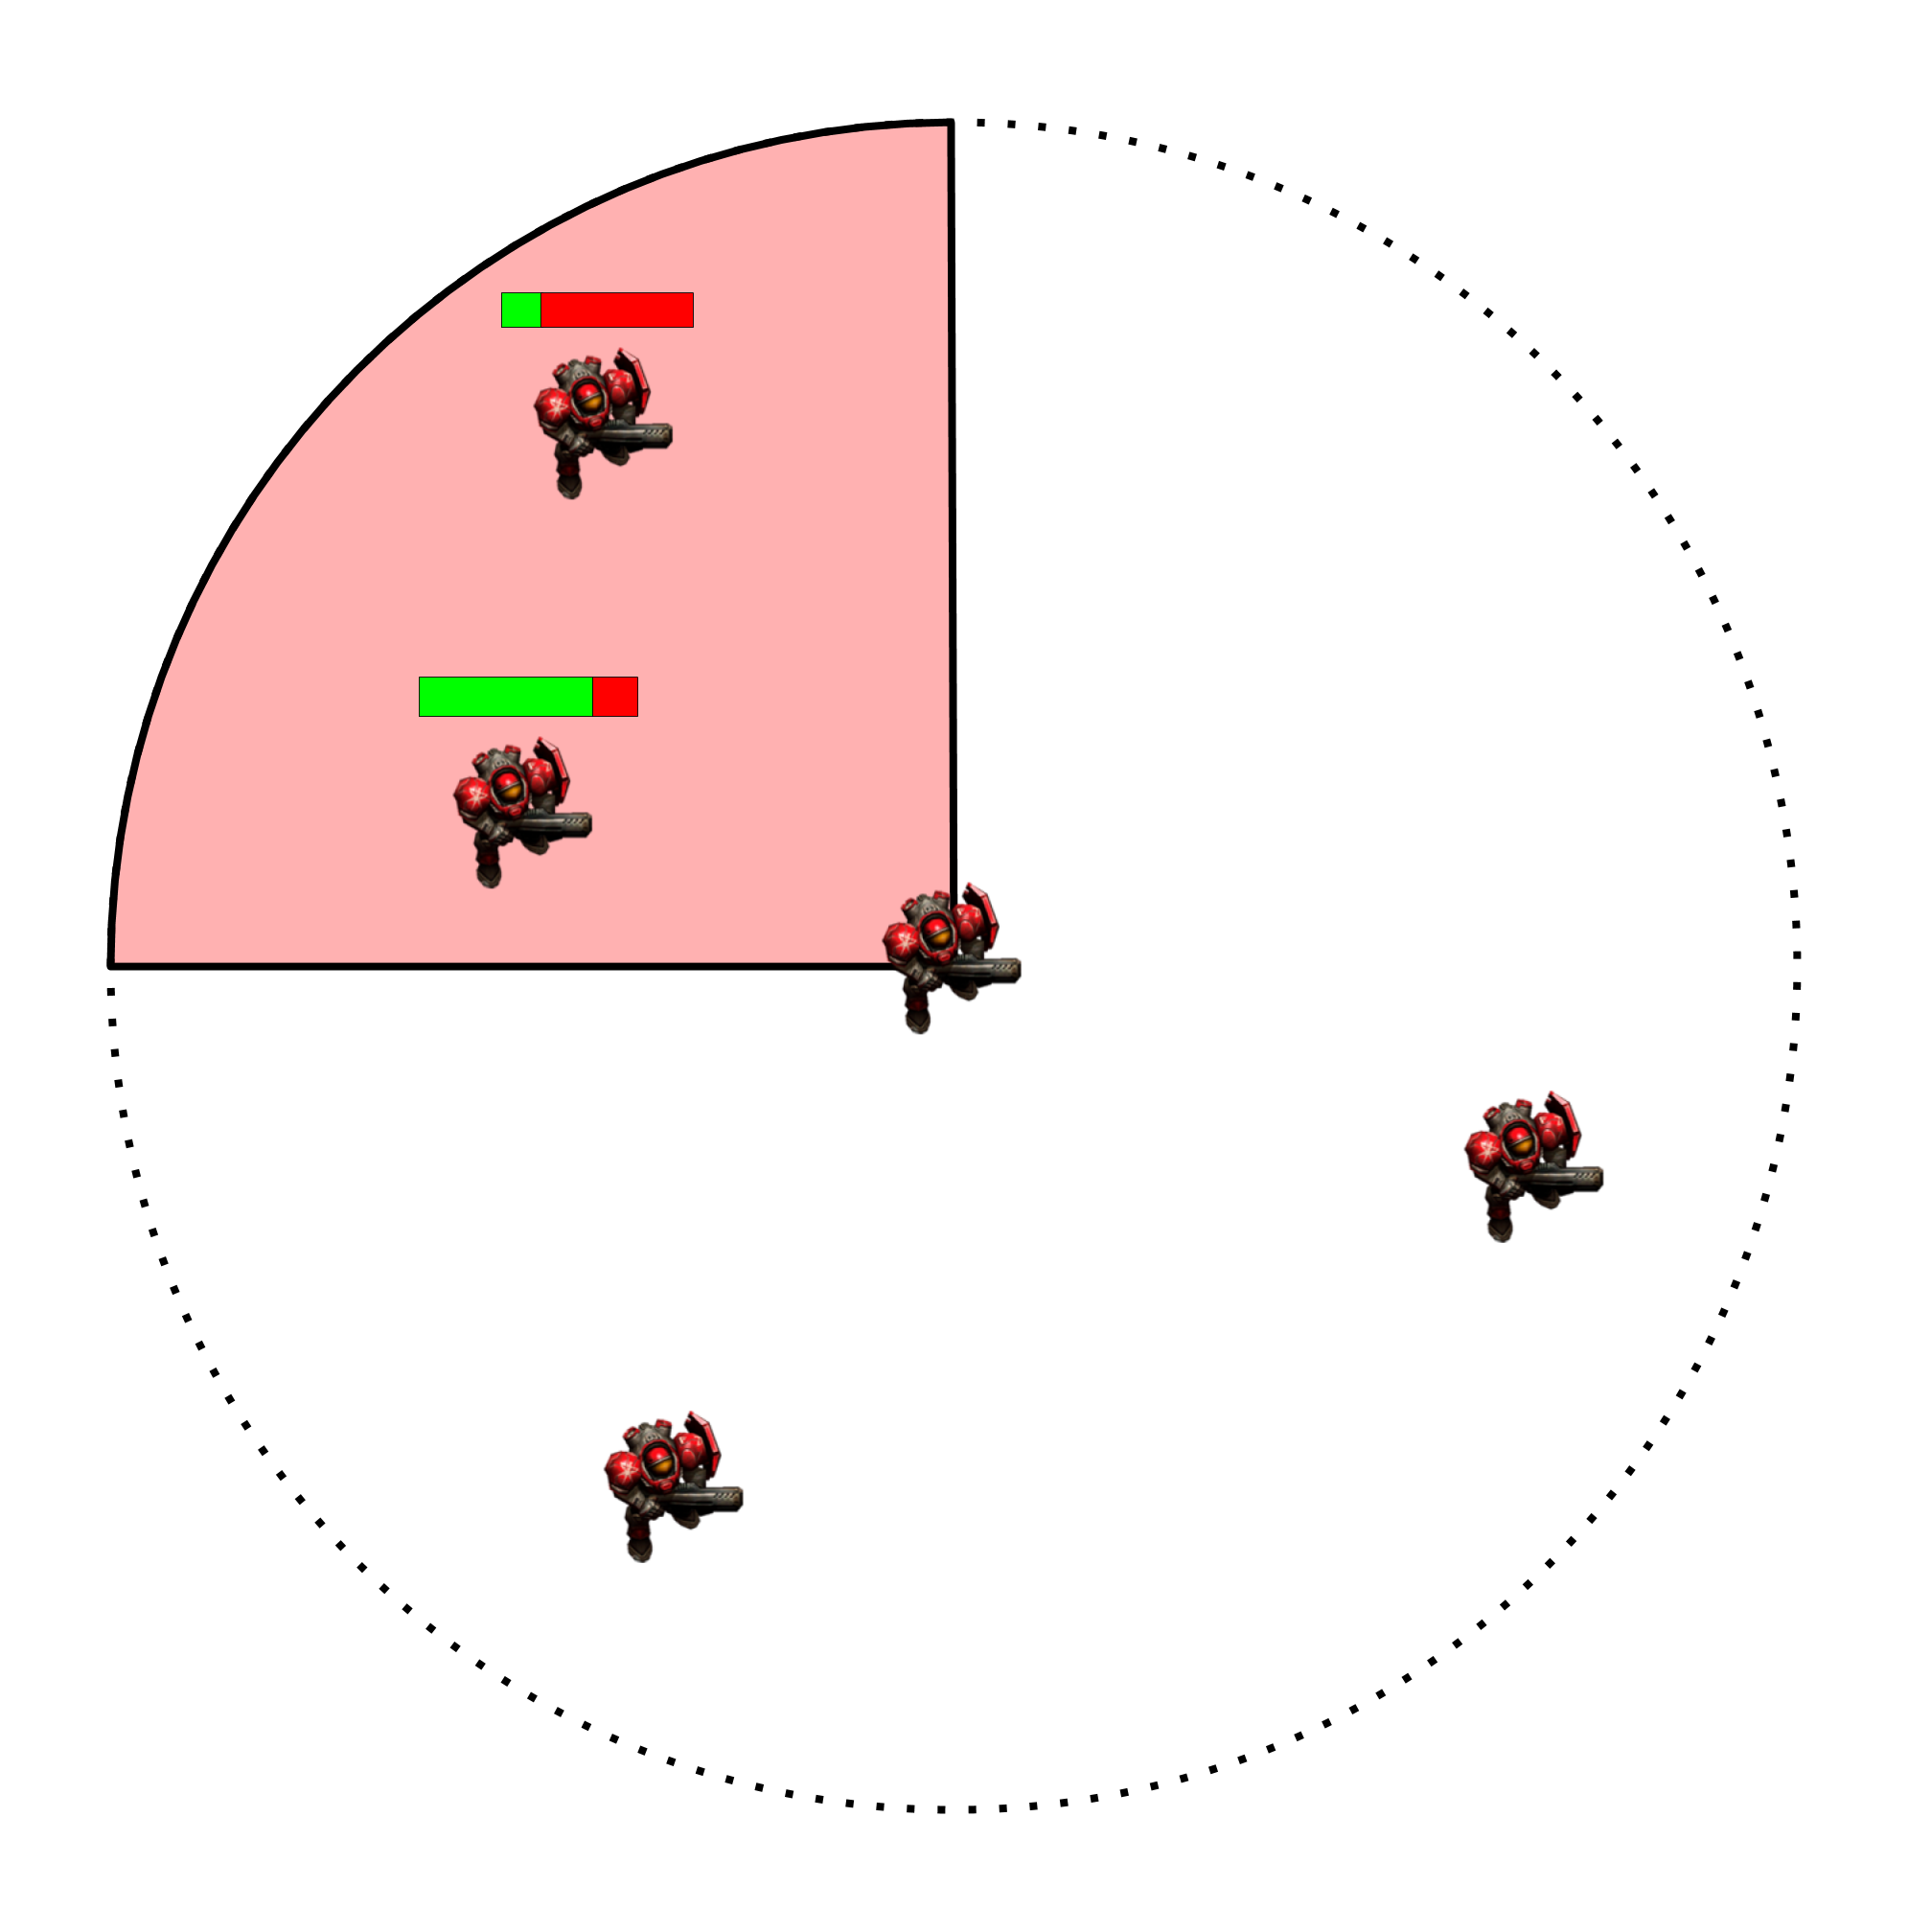
\includegraphics[width=0.6\textwidth]{ch4/discrete_state}
    \caption{Discretisation of state based on units health points.}
    \label{fig:discrete_state}
\end{figure}

We chose to approximate the state by discretise a potential function
\citep{diebelthrun} based on the health points of in-game units relative to a
particular selected allied unit (Figure \ref{fig:discrete_state}). This was
achieved by taking a particular unit as reference, filtering out everything
lying outside of the visible pixel radius, splitting then the obtained space
into a variable amount of slices. The value of each slice was then calculated by
obtaining the sum of all health ``value'' assigned to each unit within a space.
Given slice $p$ and $U_p$ units, the slice value $SV(p)$ is computed as

\begin{equation}
  \begin{aligned}
    SV(p, \beta) = & 
    \begin{cases}
      \sum_{u \in U_p}{UV(u)} & \text{if } \sum_{u \in U_p}{UV(u)} < \beta \\
      \beta & otherwise\\
    \end{cases}, \\ \text{where } 
    UH(u) = &
    \begin{cases}
      1 & \text{if } \text{health}_u < 50\%\\
      2 & otherwise \\
    \end{cases} 
  \end{aligned}
\end{equation}

We created a pair of partitions for each class of unit representing allied units
and enemy units, and added to the top the value of the reference unit health,
ending up with a relatively large tensor as our index for our action-value
function (Figure \ref{fig:array_state}).

\begin{figure}[h]
    \centering
    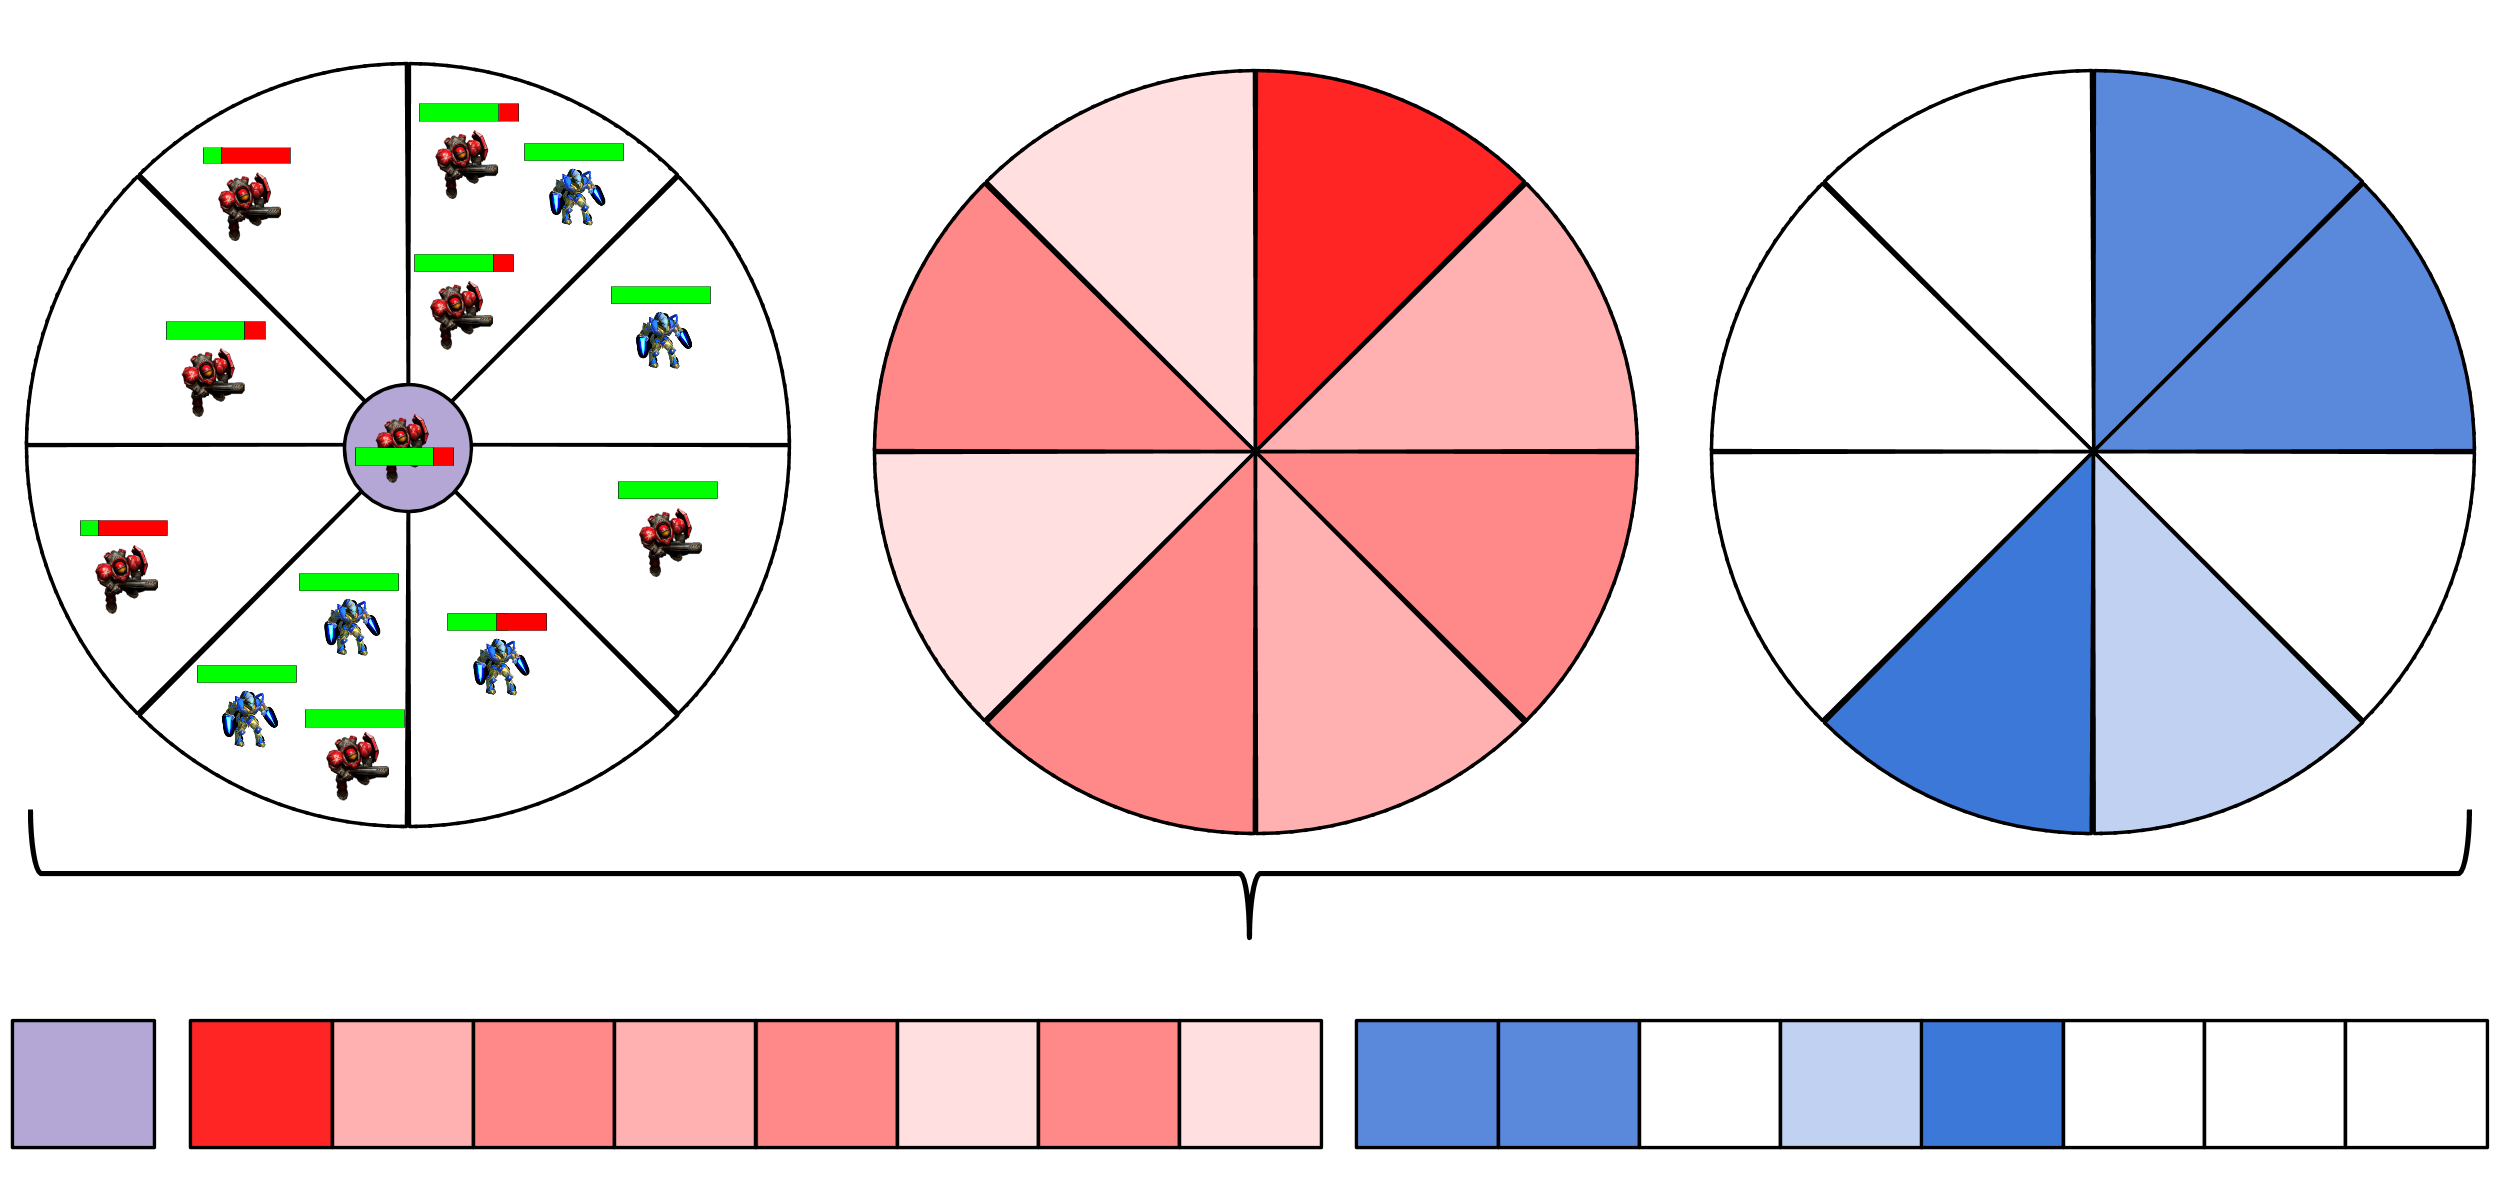
\includegraphics[width=\textwidth]{ch4/array_state}
    \caption{Mapping from slices to index tensor.}
    \label{fig:array_state}
\end{figure}

We could have also used a tile-coding technique\citep{sherstov2005function} to
stack multiple partitions of the same space (but different starting points) and
increase the generality of our state representation, but we didn't have the time
to finish its implementation.

This final technique is reasonable (as tests later confirmed) for our task, but
it wouldn't necessarily lend itself well to other scenarios. Our representation
for instance entirely lacks information about upgrades, bullets, visibility of
the map and state of the fog of war. It must be noted that with this
representation the problem becomes somewhat more complex than a standard MDP, as
we are not using the entirety of the available state information by filtering
everything outside of the image radius. We could have also used an observation
window to solve the partial observability problem, but we hypothesised that we
would obtain a good enough (but almost certainly suboptimal) policy in any case.

\subsection{Deep Q-learning}

The work described in this section is partially motivated by recent advances in
work that uses non-linear function approximators for reinforcement learning. The
\emph{Deep Q-Network} (DQN) algorithm \citep{mnih2013playing, mnih2015human} has
become one of the most popular variants of deep reinforcement learning, a
``new'' branch of reinforcement learning research that uses multi-layer ``deep''
neural networks (and other deep learning techniques) as functions approximators
to aid the decision-making process. They released their implementation together
with their Nature paper, both of which we used as a reference to develop a
version of DQN compatible with our interface.

DQN works by approximating the action-value function $Q(s, a)$ with a
Convolutional Neural Network. The network takes as input the state (in our case,
the screen image) and returns an array of values of the same size as the number
of available actions initialised when creating the network. The
$\epsilon$-greedy policy then chooses the action whose output value is highest,
or occasionally another random action.

\begin{figure}[h]
    \centering
    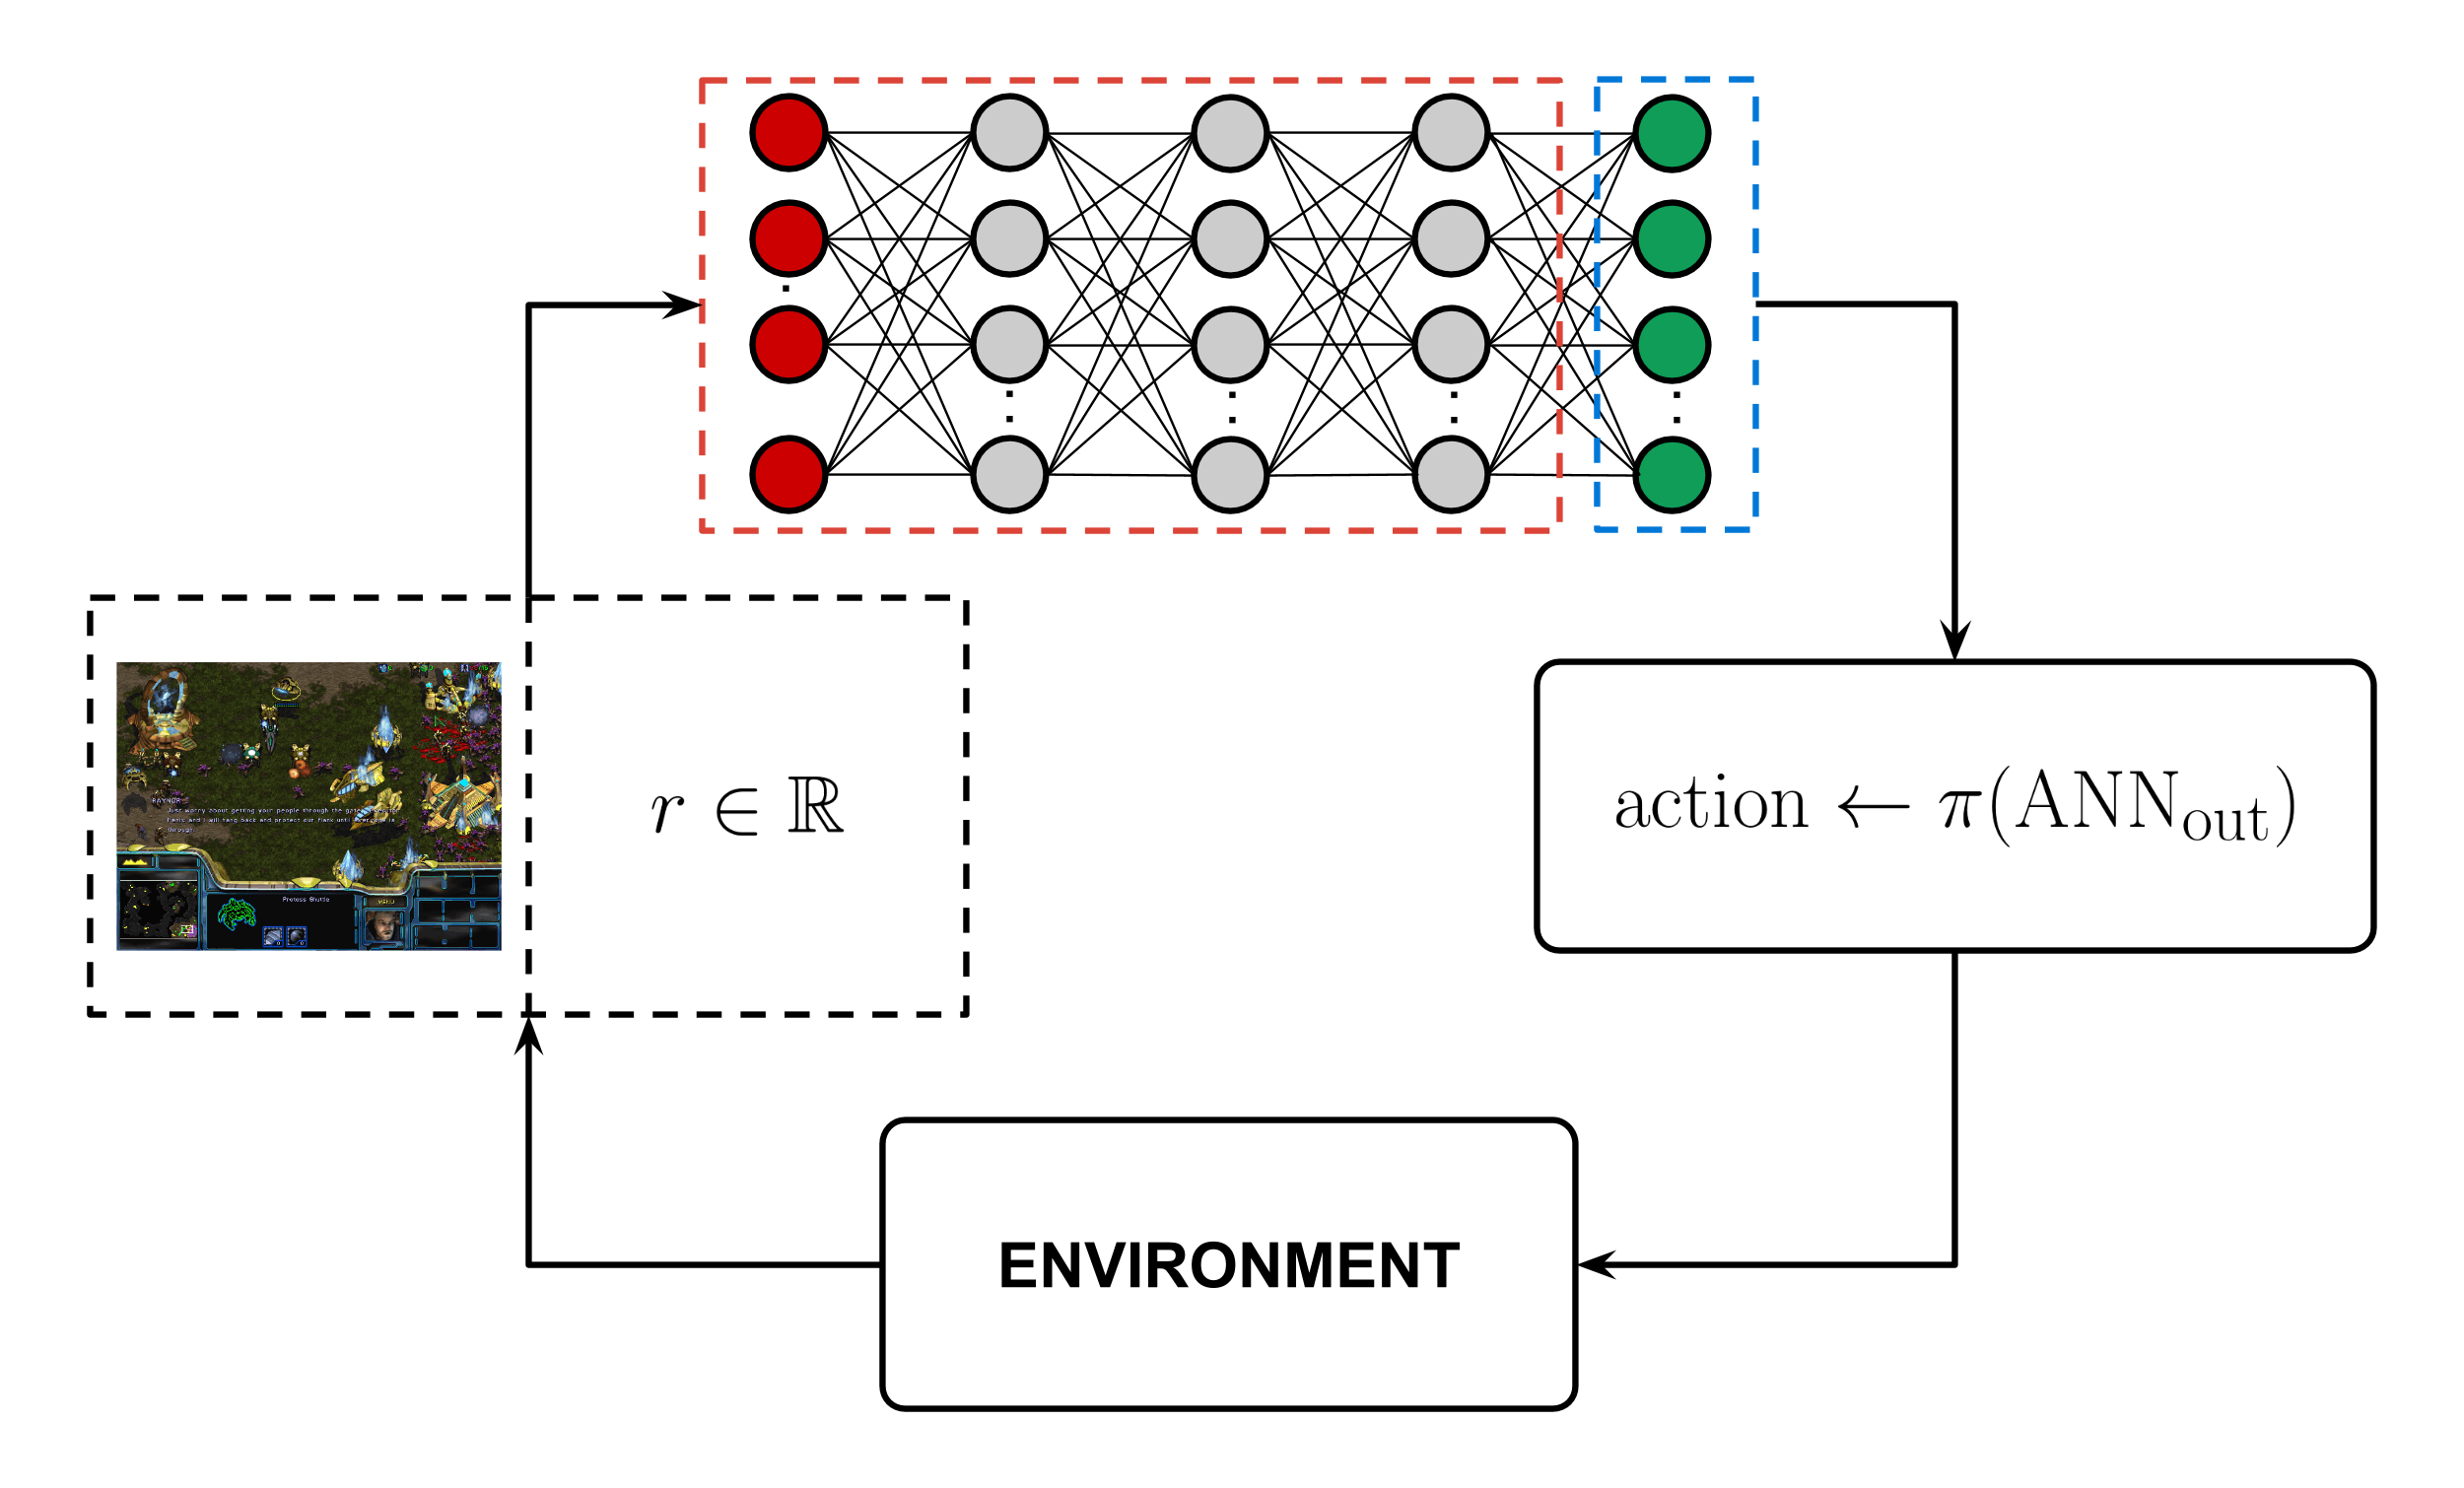
\includegraphics[width=\textwidth]{ch4/dqn}
    \caption{Deep Q-learning setting. The network outputs a value for each of
      the actions, which the policy can then use to select the preferred
      one to take.}
    \label{fig:dqn}
\end{figure}

If we consider the problem in a supervised learning fashion and imagine our
input dataset as just being generated by the interaction with the environment,
this setting then essentially becomes a regression problem with a neural
network trained using stochastic gradient descent algorithm that uses the
Q-learning update (Equation \ref{eq:ql}) as the loss function.

% TODO maybe put algorithm in here

Similarly to \cite{mnih_et_al}, our algorithms records all the tuples containing
the experience of the agent, keeps track of the newest ones using a circular
buffer, and samples from the buffer whenever the update step is called. This
functionality is called \textbf{Experience Replay} and removes the correlation
in the sequential observations, reducing the forgetting rate in the network. To
further reduce this correlation, the algorithm calculates the
temporal-difference error using a copy of the Q-network that is saved every now
and then. Finally in addition we added a maximum cap value to the
temporal-difference error to reduce big outliers and stop the weights from
changing too much when those appear.

\subsection{Multi-unit RL}

In the previous two sections we purposely avoided discussing an important design
problem related to our agent setting: by default they assume that the controlled
unit is one, while instead in StarCraft the player usually has to independently
control multiple units.

\begin{figure}[h]
    \centering
    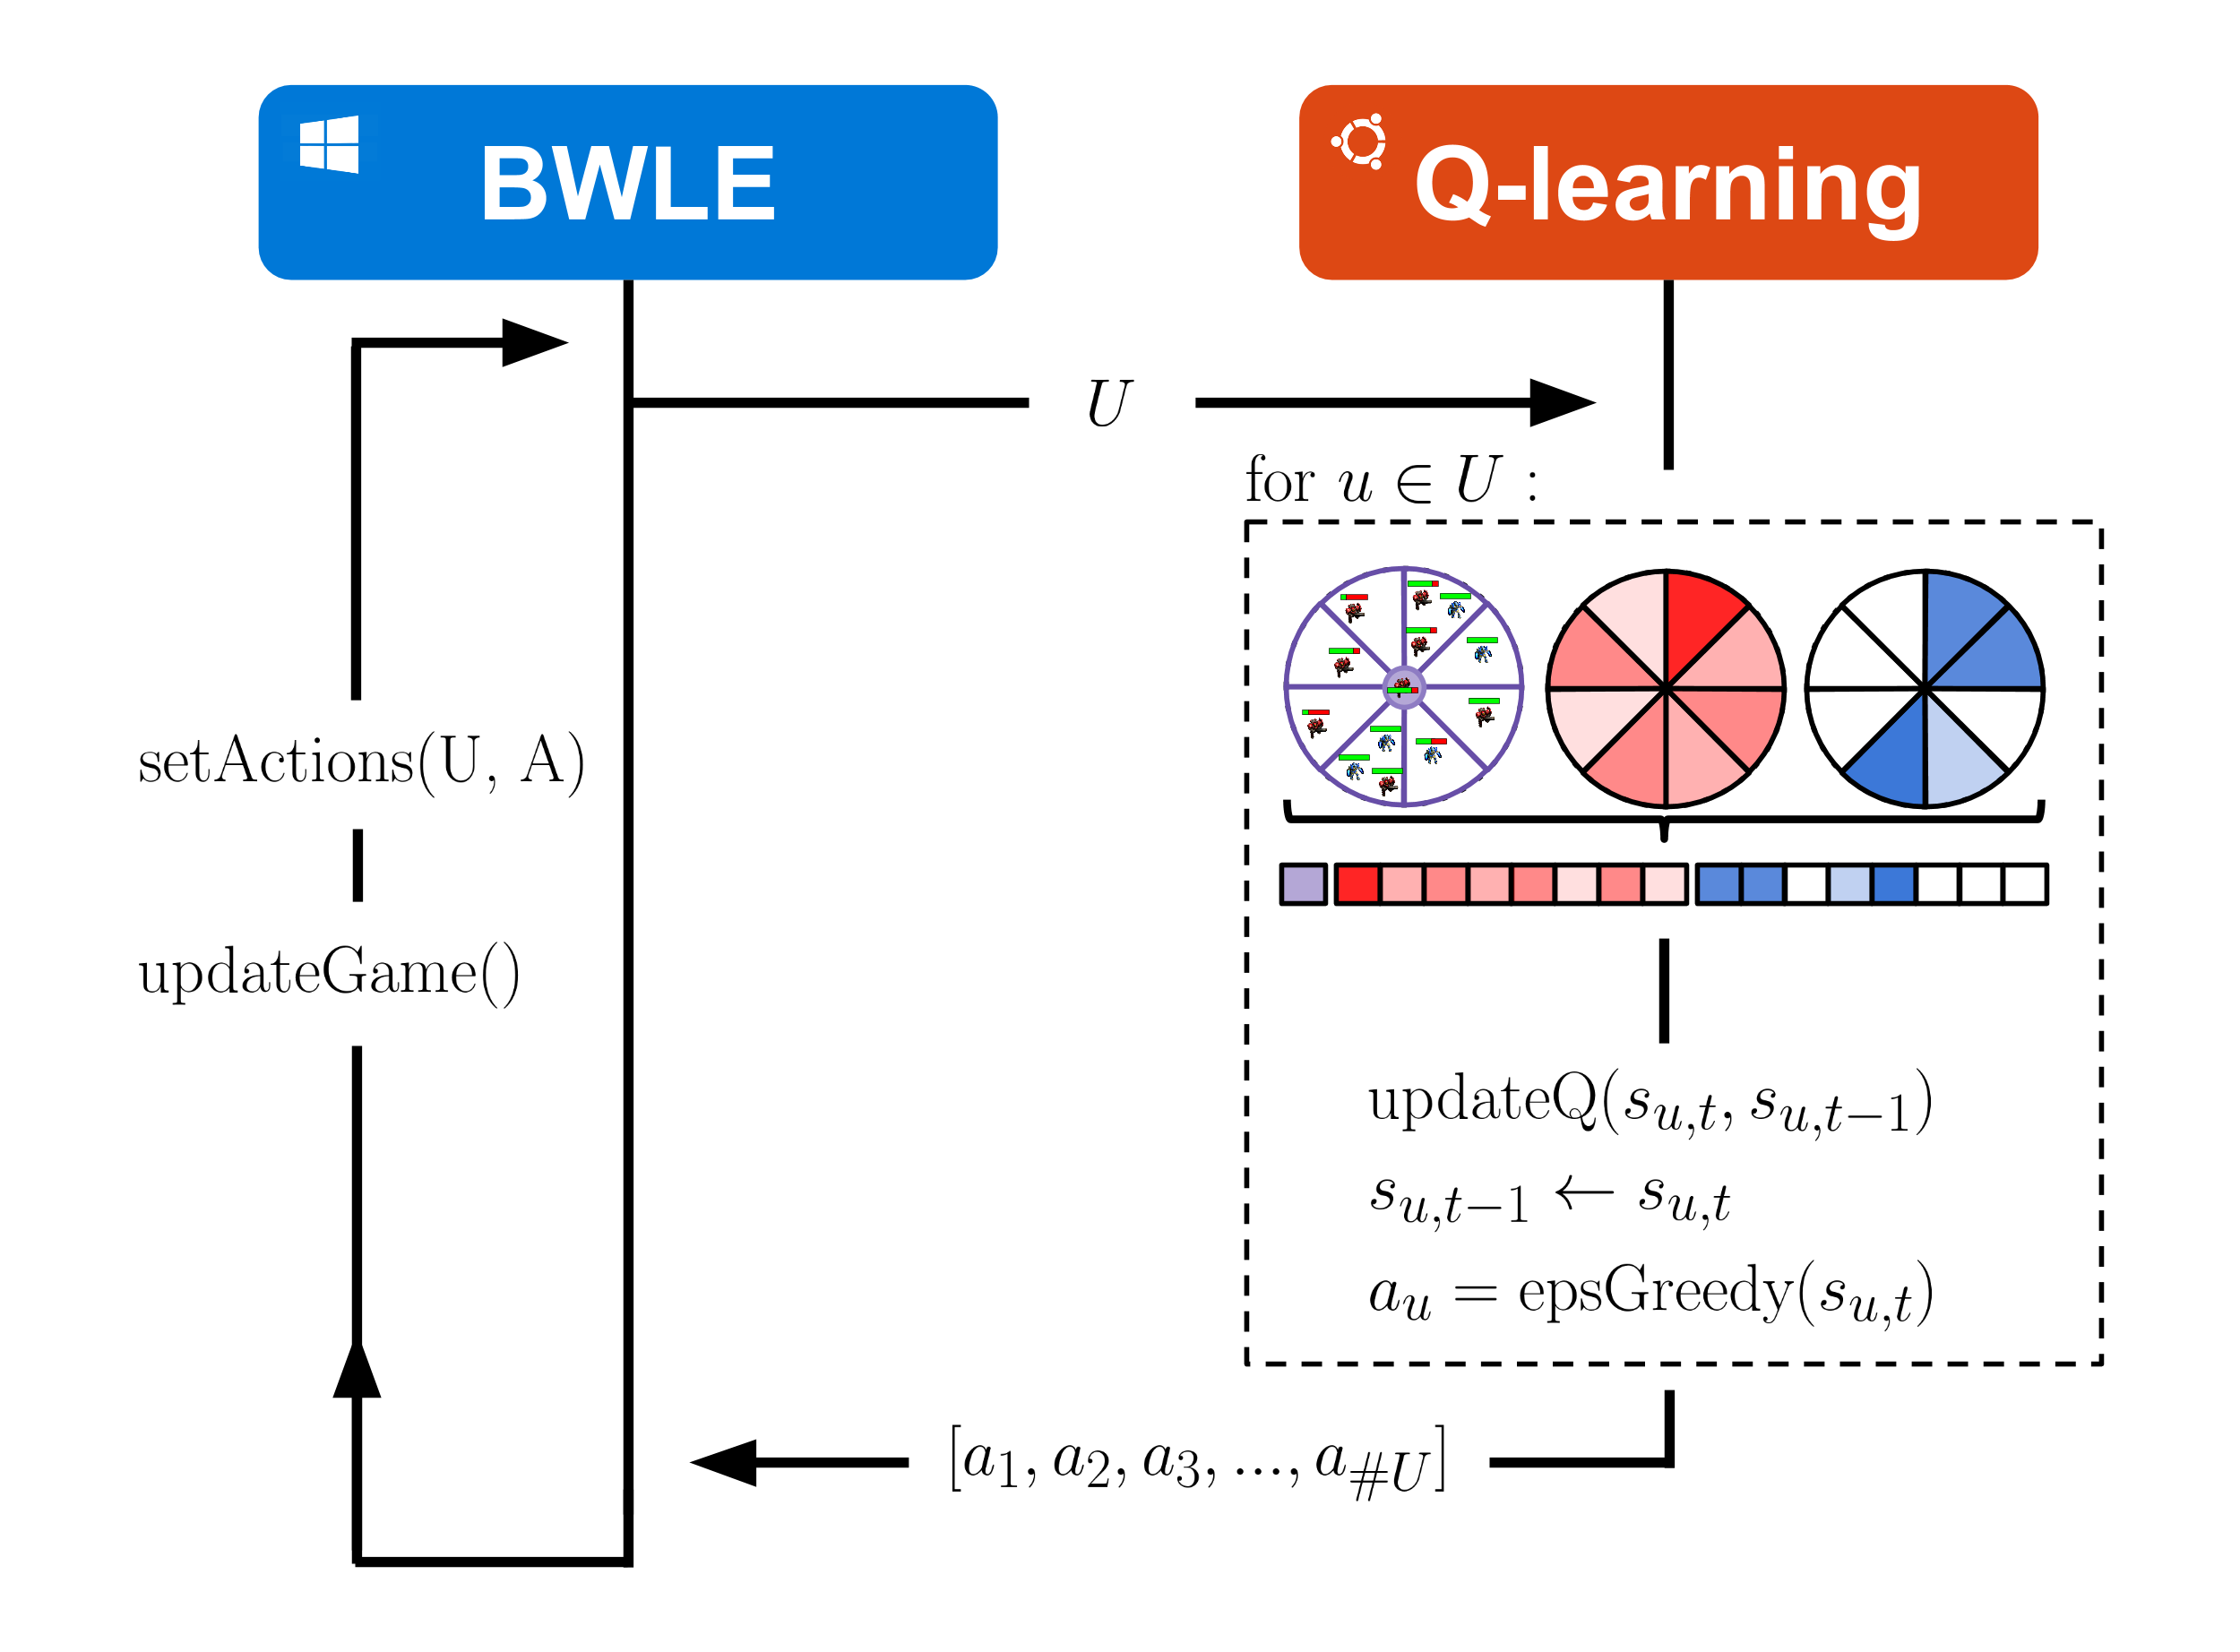
\includegraphics[width=0.9\textwidth]{ch4/parallelq}
    \caption{Visualisation of the parallel system for Q-learning.}
    \label{fig:parallelq}
\end{figure}

We didn't manage to find the time to review and implement multi-agent
reinforcement learning algorithms, so we decide to handle those multi-unit
scenarios in both Q-learning and Deep Q-learning by tweaking the
agent-environment settings.

The most effective way to coherently allow our algorithms to use multiple units
at the same time would have been to parametrise the actions by units ids, but
the actions space would then quickly explode. Additionally both our algorithms
(or at least their implementations) require the action number to be known a
priori. To avoid having to deal with the issue, we came up with a system to
optimise the execution of each unit action by parallelising the decision process
using the duration of the commanded primitive as a time buffer.

Q-learning was the easy to adapt, as the only required change to the algorithm
was to generate the state with respective to selected units and to parametrise
the action array by unit (Figure \ref{fig:parallelq}). Deep Q-learning was
harder to adapt because we had to take into account the visual window state. In
particular, to minimise the pixel variance we had to order the client to
position the window viewpoint on top of the unit to always keep it at the center
of the screen (Figure \ref{fig:paralleldq}).

\begin{figure}[h]
    \centering
    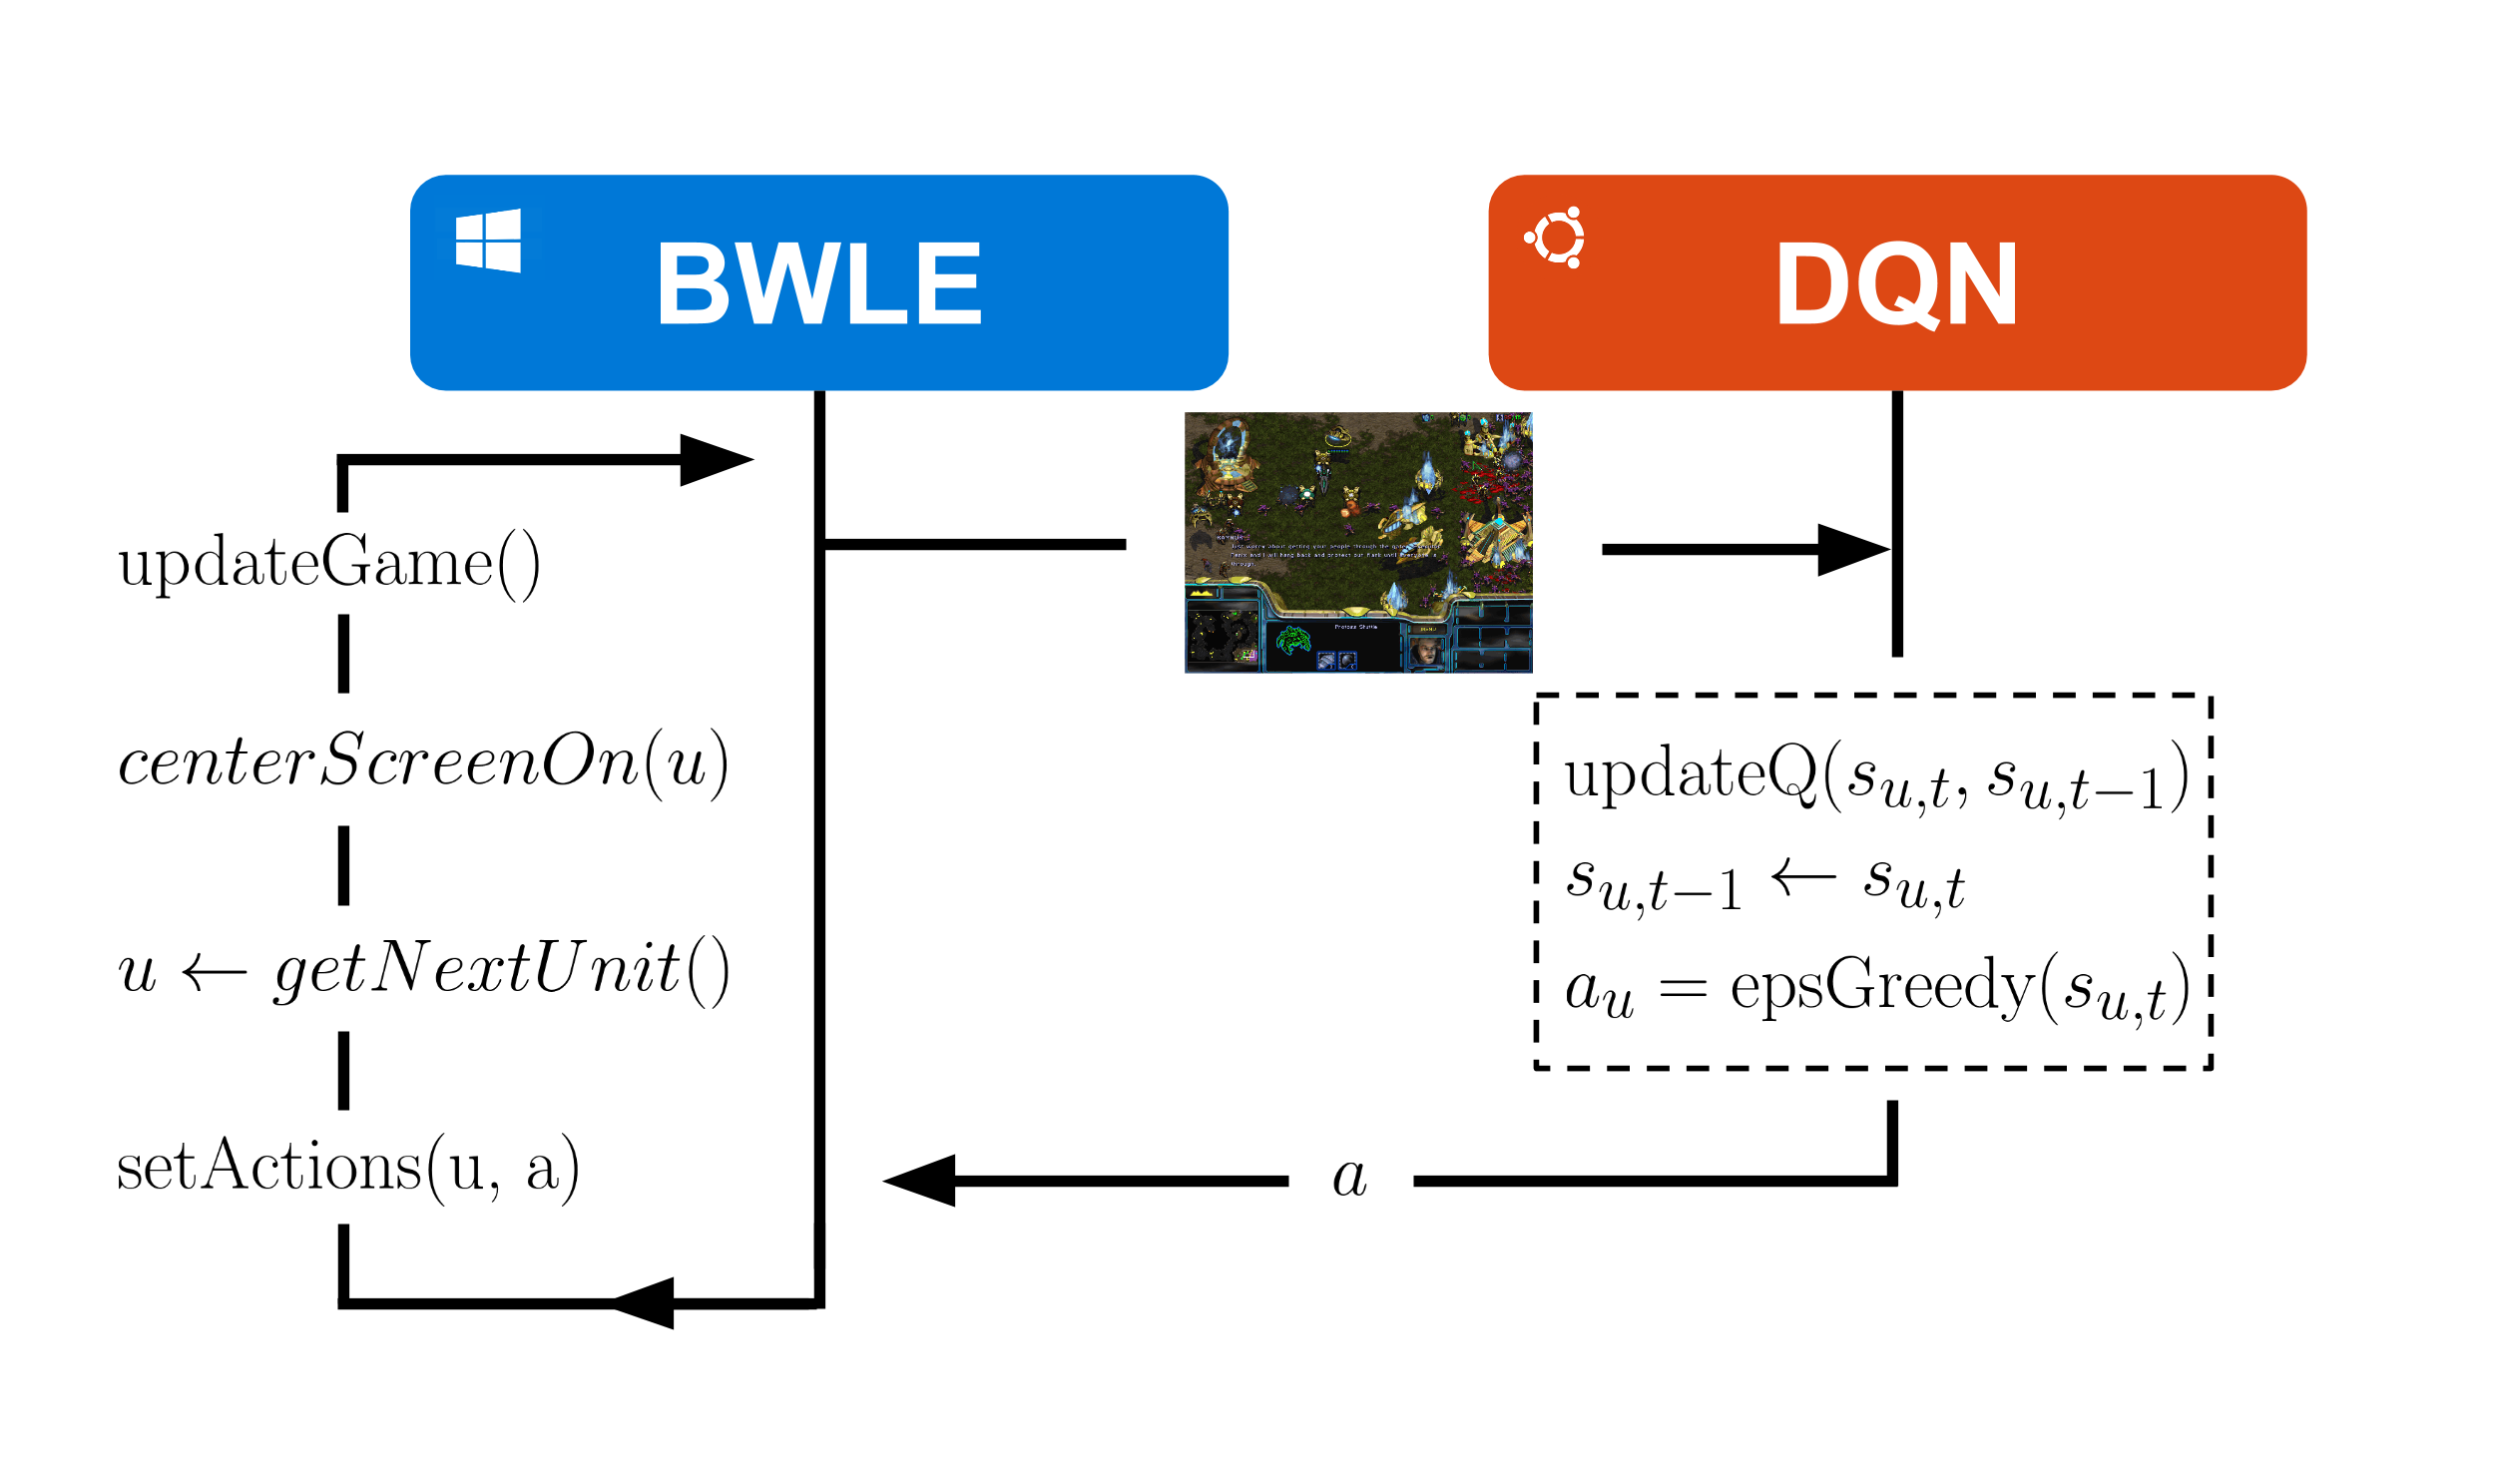
\includegraphics[width=0.9\textwidth]{ch4/paralleldqn}
    \caption{Visualisation of the parallel system for Deep Q-learning.}
    \label{fig:paralleldqn}
\end{figure}

This had the additional unexpected consequence of further randomising our
experiments, therefore allowing us to explore the state space much more quickly.
Unfortunately it also meant that the agent would not have any information about
the effect of its previous units' action choices over its future observations,
making the behaviour of allied units somewhat correlated with the agent policy.

% TODO maybe add that we had no way to check for this.

\section{Hardware Setup}

TODO. % experimental 
\chapter{Results}

\section{Stress Tests}

When we started developing BWLE we were aware of experiments running on ALE
spawning entire days \citep{mnih2015human}. Because of the huge amount of steps
steps required to learning policies based on some deep architecture, we decided
it was worth run a few stress-tests. The experiment consisted in having a basic
agent send random actions to many units for 5 million steps. We used the
synchronous communication system and fixed the observation-action rate per
minute to 600 (10 Hz), ordering the client to restart the game every 10000
iterations. The map consisted in an empty plane with a few unkillable
controllable units and the same amount of unkillable aggressive enemy unit (as
to force the game to do at least some planning all the time).

\begin{figure}[h]
    \centering
    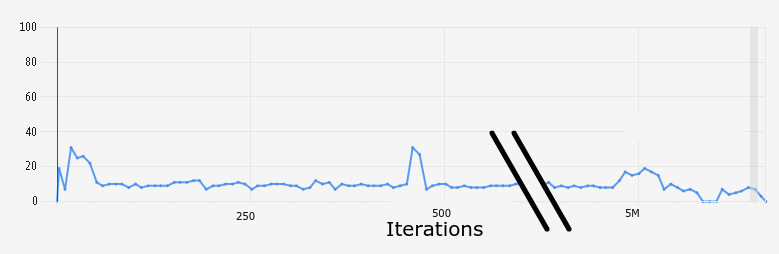
\includegraphics[width=\textwidth]{ch5/cpu_test_re}
    \caption{CPU usage of BWLE with respect to the Windows client and the Linux
      server. All the usage and was synchronously recorded every 10 steps. The
      memory usage is not shown because it completely overlaps with the CPU
      usage.}
    \label{fig:fst_usage}
\end{figure}

In terms of efficiency, Figure \ref{fig:tree} shows that the client spends the
majority of the time in idle waiting for action messages from the agent server.
For an hour we allowed the interface to run as fast as possible, reaching 18
``iterations per seconds'' when sending the image and 24 when sending only the
game state.  

\begin{figure}[h]
    \centering
    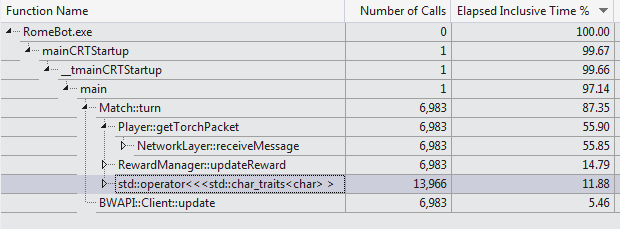
\includegraphics[width=0.7\textwidth]{ch5/client_split}
    \caption{Output of the Visual Studio 2013 C++ Profiler showing the most used
      calls in the Windows client. Ignoring the calls made to the stream
      operators (as we already provide a way to disable all printing from BWLE's
      configuration), we can see that the client spends most of the time waiting
      for responses from the server.} 
    \label{fig:tree}
\end{figure}


The recorded usage (Figure \ref{fig:fst_usage}) shows a completely stable system
that can deal with both simple and complex maps using relatively few
computational resources. We did not achieve 100\% of branch coverage because we
didn't allow the usage of all the available actions, but the majority of the
client available interface was called at least once (in particular, according to
Visual Studio 2013 90\% of branch coverage was reached).

It must also be noted that most StarCraft AI tournaments
\citep{ontanon2013survey} run BWAPI-based clients for entire weeks without any
noticeable problem, so the results we obtained were not unexpected.

\section{Navigation Task}

Next we tested our algorithms on the first StarCraft task, the``Navigation
Task''. The obtained results mostly matched our expectations: the task consisted
essentially in a medium-size grid-world which both algorithms managed to
eventually converge. Figure \ref{fig:nav_task_results} shows the average reward
per episode, where an episode is defined as the sequence of steps from the
starting state to a terminal state. The policies were evaluated every 10000
iterations by playing 10 episodes, recording mean and standard deviation.

\begin{figure}[h]
    \centering
    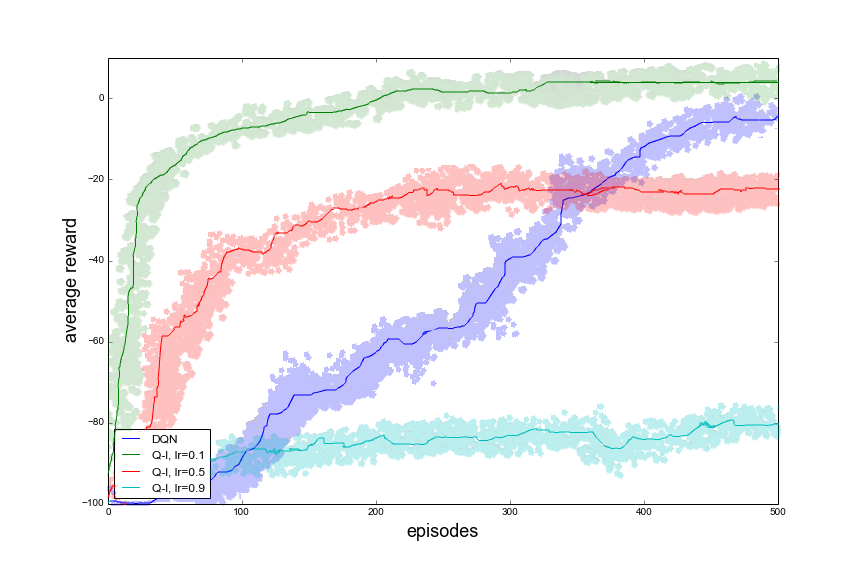
\includegraphics[width=\textwidth]{ch5/nav_task_re}
    \caption{Results of DQN and Q-learning on the simpler navigation task.}
    \label{fig:nav_task_results}
\end{figure}

Q-learning was tested with three different learning rates, while DQN was tested
using the same parameters used in \cite{mnih2015human}. We tried to do a more
appropriate sweep in the parameters space, but DQN tended to diverge when
varying too much some of the parameters and it would have taken too much time to
proceed with additional testing. Changing the action persistence window size
significantly impacted the learning process, as small windows made movement
actions too quick for the agent to switch from one block of the grid to the
other, rendering the task partially observable. We know that while DQN is stable
for MDPs, states with imperfect information in general require some stochastic
strategies to reach policies that are close to being optimal
\citep{heinrich2016deep}.

\section{Guided Navigation Task}

The experimental setting was similar to the previous experiment, beside having a
different map and reward function. DQN was trained using all the 20 available
maps, while Q-learning had to learn exclusively one map. This choice was made to
avoid having to find the correct parameters values, as the map was much larger
and we couldn't feasibly decrease the resolution of the grid without changing
the map's walkable paths average width.

\begin{figure}[h]
    \centering
    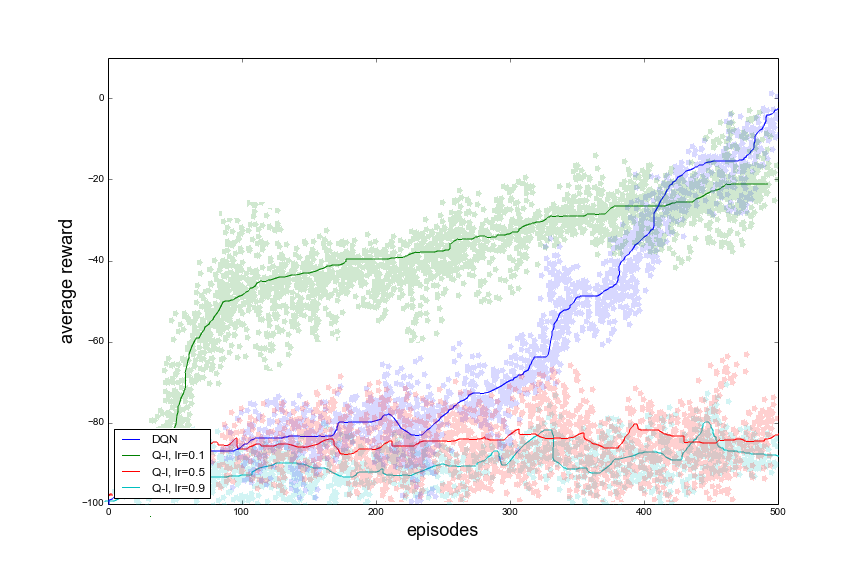
\includegraphics[width=\textwidth]{ch5/guid_task_re}
    \caption{Results of DQN and Q-learning on the guided navigation task.}
    \label{fig:guid_task_results}
\end{figure}

Figure \ref{fig:guid_task_results} shows the learning curve similarly to the
previous experiments. We can see that after around 400000 iterations the total
reward starts to converge.

\section{Survival Task}

Our last experimental setting was also the hardest. We hypothesised that both
algorithms would learn to survive by fighting, but we also expected the CNN to
acquire policies invariant to the units positions and more correlated to the
amount of units. We also expected to see more variance at evaluation time due to
the uneven difficulty of the designed maps.

% TODO Write the need to remove outliers.

Figure \ref{fig:surv_task_results} shows the results obtained by running
multi-unit Q-learning and multi-unit DQN. As predicted, the standard deviation
of the episodic reward arrays ended up being much higher compared to the other
tasks because some of the maps were significantly harder than others (as some
units were doomed to die). We can see that the average amount of steps in an
episode gradually increases, which means that learning is happening.

\begin{figure}[h]
    \centering
    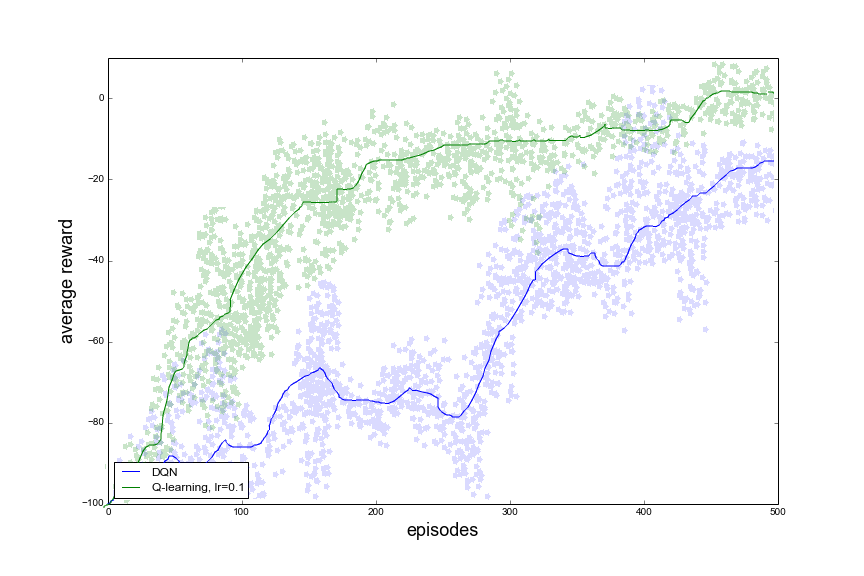
\includegraphics[width=\textwidth]{ch5/surv_task_re}
    \caption{Results of DQN and Q-learning on the harder Survival task.}
    \label{fig:surv_task_results}
\end{figure}

We inspected the collected action data and we noticed that the distribution of
actions taken by each unit differed significantly depending on the amount of
allied and enemy units. This was probably due to the fact that the Convolutional
Neural Network built filters invariant to the position of the units, making it
more likely to try and shoot other units when close to allied units. Finally,
at the end of the training session, the units lasted on average 50 iterations
more than at before training.

\section{Chapter Summary}

In this chapter we presented the results of the experiments described in Chapter
4. We confirmed some of our initial hypotheses and tested the platform to its
limits, providing a baseline for future design and research work.
 % results
% outline discussion
% 1. Symbolic restructuring
% 2. DQN results 
% 3. Problems with StarCraft
% 4. Can we make the interface better? 

\chapter{Discussion}

\section{Framework Evaluation}

The initial idea was to create modules to cluster part of the useful game state
in such a way that researchers would have only needed to ``configure'' a reward
function (if needed). Moreover one of the first design decisions turned out to
be slightly detrimental when we switched to the multi-client architecture,
making the implementation unnecessarily tricky and bug-prone.

When we came up with the project we weren't expecting to spend so much time on
it. 

Over the course of the project we have realised that StarCraft is challenging
for a large variety of reasons, most of which shared with a lot of other RTS
games but also inherently due to the platform itself. We couldn't have done much
better using any of the other available RTS games (and BWAPI is so good that
without it we would have definitely not been able to carry on this project).
 
\subsection{How can we improve this?}

The easiest but most painful solution (implementation-wise) to the design
problem would be to partially re-design the way the client handles the game,
while leaving the interface unchanged.

This could be achieved in different ways:

\begin{itemize}
\item The client could be split in three different asynchronous modules: a
  StarCraft handler to control Windows and the StarCraft process, a Game State
  collector to observe and collect the state using BWAPI and WinAPI, and a
  networking interface to deal with the external interface.
\item BWAPIClient could be expanded to fully control the game in a similar
  fashion.
\end{itemize}

\section{Challenges for machine learning approaches}

\subsection{State exploration as a policy}

\subsection{Hierarchical Decision-Making}

In Chapter 2 we have discussed some work in Hierarchical Reinforcement Learning
that could be used in principle to tackle StarCraft, however no particular model
seems to fit all the requirements of the platform, especially if we take and
end-to-end approach to the problem. It's probably fair to speculate that
similarly to AlphaGo, a reinforcement learning framework will need some amount
of strong supervision to learn good overall strategies and hand-tuned feature
extractors.

% Cover Russell work

\section{Future Work}

\subsection{Full Linux compatibility}

The great majority of AI and machine learning researchers do not use Windows as
their development environment. Having to use a VM to host the StarCraft client
and the interface means that there is a higher cost then normal associated with
using the platform (i.e. it's not straightforward to provide a simple
installation script or a working out-the-box environment).

In the past some parts of BWAPI were compatible with the WINE, a Linux
environment that tries to reproduce the Windows API and provide tools for
running Windows software on unix platforms. Porting the entirety of our pipeline
over Linux will mean being able to significantly simplify the integration with
other state-of-the-art machine learning systems. 

\subsection{ROS integration}

% picoros

% ros 2.0


\subsection{Policy Reuse}

% include also policy distillation? % discussion
% outline conclusion
% 1. Conclusion of scoping work

\chapter{Conclusion}

Finally reaching the end of this project, we can say that we have reached an
extremely satisfactory point in the development of a new agent learning
platform. Not only we have met and gone past our initial engineering goals, but
we have also managed to show that it is possible to learn interesting policies
using both standard Q-learning and Deep Q-learning when StarCraft is reduced
into a simple MDP setting, and we have lain down the algorithmic baseline for
our next experiments in the area. We now believe that it is essential we start
designing policies with hierarchical structures in mind from the start.

Designing, implementing and testing the platform took well over 800 hours, while
a couple of other hundreds of hours were spent reproducing different
implementations of Q-learning and Deep Q-networks. Unfortunately a lot of time
was spent refactoring and dealing with the complex - and sometimes buggy -
behaviour of Windows APIs and StarCraft, however our efforts paid off by giving
us an extensible and useful platform.
 % conclusion

\bibliographystyle{plainnat}
\bibliography{thesis}

\end{document}

